\section{Einführung}
Das Heinrich-Hertz-Europakolleg Bonn verlangt im fünften und sechsten Semester
der Weiterbildung zum staatlich geprüften Informatiker eine fachbezogene
Projektarbeit. Dieses Projekt wird in Gruppen von zwei bis vier Personen
durchgeführt und soll fachliche Inhalte sowie Inhalte aus dem Projektmanagement
kombinieren. Es handelt sich um eine praktische Arbeit. Jeder Abschnitt enthält
ein Kürzel des Autors, hierbei bedeutet:
\begin{outline}
  \1 {[MR]} erstellt von Marcel Reuter
  \1 {[NL]} erstellt von Nikolai Luis
  \1 {[TM]} erstellt von Tim Meusel
\end{outline}
\tm%

\section{Projektvorstellung}
\label{subsubsec:projektvorstellung}
Cloud Provider bieten verschiedenste virtuelle Instanzen auf physischen Hosts
an. Dabei nutzt jeder virtuelle Server die vorhandenen Ressourcen des
physischen Systems unterschiedlich. Hier kommt es, aufgrund der
Mischkalkulation für die Ressourcen, zu einer Überbuchung (Overcommitment) des
Hosts. Weil das Monitoring nicht ausreichend ist, oder kein sinnvolles
Placement implementiert ist (Placement beschreibt den Algorithmus der einen
Node ermittelt auf dem eine neue virtuelle Instanz angelegt wird) kommt es
regelmäßig zu Performanceeinbußen. Für Kunden gibt es keine Transparenz über
die ihm zugeteilten und durch ihn genutzten Ressourcen, weshalb auch keine
ressourcenbasierte Abrechnung erfolgen kann. Teamleiter sind häufig mit der
Effizienzsteigerung der Plattform beschäftigt und müssen die Auslastung
steigern. Dies ist ohne detaillierte Auslastungsreports nicht möglich.

In diesem Projekt soll eine funktionierende Open Source Software entwickelt
werden, die sich in drei Teile gliedert:
\begin{outline}
  \1 Die verschiedenen Ressourcetypen (CPU Zeit / Datendurchsatz / RAM
  Auslastung / Speicher Auslastung / Netzwerkdurchsatz) der einzelnen
  virtuellen Server müssen in einem sinnvollen Intervall periodisch ermittelt
  werden.
  \1 Die Daten müssen aggregiert und gespeichert werden. Hierbei ist auf eine
  Skalierung auf mindestens 10.000 virtuelle Instanzen unter Berücksichtigung
  der Verfügbarkeit und Performance der Datenbank zu achten (Sharding oder
  Replikation, verteilt oder zentral, dokumentenbasiert oder relational).
  \1 Diese Daten können dann dem Endanwender präsentiert werden (\gls{API} und
  Web-UI). Hierzu wird eine Userstory Erhebung unter den drei Anwendertypen
  Kunde, Administrator, Manager bei Partnerunternehmen durchgeführt, um
  gewünschte Algorithmen zur Visualisierung zu ermitteln (zum Beispiel
  ermitteln von freien oder überbuchten Nodes, grafische Auswertung für Kunden).
\end{outline}

Dieses Projekt eignet sich besonders gut als Projektarbeit, da es in drei Teile
gegliedert ist. Jeder dieser Teile ist eigenständig und wird einem
Projektmitglied zugeordnet. Dies erleichtert die spätere Bewertung.
\tm%

\subsection{Projektteam}
Das Projektteam besteht aus den drei Mitgliedern Marcel Reuter, Nikolai Luis
und Tim Meusel.
\tm%

\subsubsection{Marcel Reuter}
Herr Reuter beendete 2013 seine Ausbildung zum IT-Systemelektroniker und
arbeitet seit dem bei der Firma EBF-EDV Beratung Föllmer GmbH. Er ist
verantwortlich für die visuelle Schnittstelle des Projekts (Punkt 3).
\mr%

\subsubsection{Nikolai Luis}
Herr Luis begann die Weiterbildung zum Techniker wärend seiner Ausbildung zum
Fachinformatiker Anwendungsentwicklung, welche er im Januar 2016 beendete. Er
arbeitet als BIG Data Analyst bei der Deutschen Telekom. Er ist verantwortlich
für die Speicherung der Daten und die automatisierte Schnittstelle (Punkt 2).
\nl%

\subsubsection{Tim Meusel}
Herr Meusel schloss seine Ausbildung zum Fachinformatiker Systemintegration
2012 ab. Aktuell arbeitet er als Systems Engineer bei der Host Europe Group.
Er verantwortet die Ermittlung sowie Übertragung der Daten.
\tm%

\subsection{Auftraggeber}
Die Ansprechpartner für dieses Projekt ist das Unternehmen Puppet Inc. (im
folgenden Puppet) in der Rolle als Auftraggeber, welches von den Mitarbeitern
Herrn David Schmitt und Herrn Steve Quin vertreten wird. Puppet ist Marktführer
im Bereich Konfigurationsmangement Software. Software dieser Art hilft es
Administratoren sehr einfach Testumgebungen aufzubauen und auch
Produktivumgebungen zu Verwalten. Das Kernprodukt der Firma Puppet, welches
ebenfalls puppet heißt, steht unter einer Open Source Lizenz und darf frei
genutzt werden. Der Einsatz der Software erlaubt es dem Projektteam
verschiedenste Prototypen in kurzer Zeit zu bauen. Puppet entwickelt außerdem
Software zum Testen. Dies vereinfacht das Qualitätsmanagement im Projekt.
Puppet hat in der Vergangenheit bewiesen, mit agiler Entwicklung und diversen
Testverfahren umgehen zu können, beides wird intensiv in deren Teams genutzt.
Herr Quin und Herr Schmitt bieten tiefgreifendes Wissen zu den verschiedenen
Programmen und Techniken, um das Projektteam zu untersützen und zu beraten.
\tm%

\subsection{Aktuelle Situation}
In der~\ref{subsubsec:projektvorstellung} wurden bereits die Intentionen des
Projekts erläutert. In der Vergangenheit wurde schon mal versucht eine passende
Softwarelösung zu entwickeln. OpenStack ist ein Softwareprojekt mit dem große
Mengen an Rechen- und Netzwerkkapazitäten, sowie persistenter Speicher in einem
Rechenzentrum zu einer \gls{Public Cloud} oder \gls{Private Cloud} Umgebung
zusammengefasst und orchestiert werden~\cite{OpenStack_Intro}. Eines der
Teilprojekte ist Telemetry. Das Ziel hiervon ist es, zuverlässig Daten von
physischen und virtuellen Ressourcen zu ermitteln verlässlich zu speichern. Die
Daten sollen zur Analyse genutzt werden und Aktionen auslösen wenn bestimmte
Kriterien erreicht sind~\cite{OpenStack_Telemetry}. Telemetry bringt leider
mehrere Nachteile mit sich:

\begin{outline}
  \1 Die Standarddatenbank für Telemetry war lange Zeit MongoDB\@. MongoDB ist
  eine dokumentenorientierte Datenbank, hier werden Daten nicht in Tabellen
  strukturiert sondern in eigenständigen Dokumenten. Jedes Dokument hat eine
  eigene Datenstruktur (z.B. im \gls{JSON}
  Format)~\cite{Dokumentenorientierte_Datenbank}. Dies ermöglicht es, die
  Datenbank sehr einfach vertikal zu skalieren. Hierbei werden alle Dokumente
  auf mehrere Server verteilt. Schreib- und Lese-Anfragen können ebenfalls auf
  alle Server verteilt werden. Die Skalierung ist nahezu
  linear~\cite{MongoDB_Architecture},~\cite{What_is_MongoDB}. Die Grundidee ist
  sehr gut und eignet sich für besonders große Datenmengen oder Installationen
  die Hochverfügbar sein müssen. Die Implementierung in MongoDB hat allerdings
  diverse Nachteile. Kyle Kingsbury hat intensiv MongoDB mit \gls{Jepsen}
  getestet. Die Datenbank hat sich mehrfach als sehr unzuverlässig
  herausgestellt~\cite{MongoDB_on_Jepsen}. Die beiden folgenden Punkte
  disqualifizieren MongoDB für einen Einsatz als persistenten  Datenspeicher,
  da die Persistenz nicht sichergestellt ist. Es wurde von Kyle Kingsbury
  bewiesen, das:
    \2 MongoDB bei einem Schreibvorgang bestätigt, das Daten persistent
    gespeichert wurden, dies allerdings nicht immer der Fall ist. Ein
    unbemerkter Datenverlust ist die Folge.
    \2 MongoDB in bestimmten Situationen die falschen Daten bei einer
    Leseanfrage zurückliefert.

  \1 Das Telemetry Projekt hat diese Probleme ebenfalls erkannt und nach
  alternativen Datenbanken gesucht. Nachdem keine vorhandene Lösung ihren
  Anforderungen entsprach, entschieden sie sich für die Entwicklung einer
  eigenen Datenbank: \gls{Gnocchi}. Diese Datenbank ist noch in der Entwicklung
  und noch nicht für den produktiven Einsatz bereit.
  \1 Es wird immer wieder von Skalierungsproblemen berichtet. Das CERN betreibt
  eine OpenStack Installation und konnte die Probleme mit Telemetry nur mit
  immenser Hardware lösen. Die Kosten für diese Infrastruktur als auch die
  Komplexität sind viel zu hoch. Sie übersteigen das Budget der meisten Cloud
  Umgebungen wodurch diese unwirtschaftlich werden~\cite{OpenStack_CERN}.
  \1 Das Telemetry Projekt ist sehr stark in OpenStack eingebunden. Der Einsatz
  in anderen Cloud Umgebungen ist nicht vorgesehen, da die einzelnen Dienste
  aus dem Telemetry Projekt weitere OpenStack Komponenten benötigen. Ein
  eigenständiger betrieb ohne OpenStack ist nicht geplant für die Zukunft.
\end{outline}

Aufgrund der langen Liste an Problemen ist Telemetry aktuell innerhalb einer
kleinen OpenStack Installation teilweise nutzbar, jedoch nicht wirtschaftlich
in großen Umgebungen oder außerhalb von Openstack. Es ist nicht davon
auszugehen, dass diese Probleme kurz- bis mittelfristig gelöst werden. Somit
entschied sich das Projektteam eine Alternative zu entwicklen die unkompliziert
zu installieren ist und unabhängig von OpenStack arbeitet.
\tm%

\subsection{Anforderungen}
Die Detailanforderungen werden getrennt für die drei Bereiche des Projekts im
folgenden Abschnitt beschrieben. Diese ergeben sich aus dem Lastenheft und
Pflichtenheft sowie aus den Userstories der Partner. Für Alle Lösungen gillt,
das sie eine aktive Community haben und unter einer Open Source Lizenz stehen.
\tm%

\subsubsection{Datenerfassungssysteme}
\label{subsubsection:datenerfassungssysteme}
Unterschiedliche Ausbaustufen für virtuelle Machinen werden über mehrere
verschiedene Ressourcen, die sich in Ihrer Leistungsklasse unterscheiden,
differenziert. Diese Typen müssen für jede virtuelle Machine ausgelesen werden.
Als Referenz werden die Typen der größten deutschen Anbieter nachweis! für
virtuelle Machinen genommen. Diese sind aktuell:

Zugewiesener Arbeitsspeicher, Anzahl/Leistung der Prozessorkerne, Durchsatz des
Datenträgers, Anbindung an das Internet, nachweis via scrots fachwörter
referenz?

Diese Werte müssen sowohl in den virtuellen Machinen als auch auf dem Host
ermittelt werden können. Im Bereich Managed Hosting hat der Hoster Zugriff in
die virtuellen Instanzen und kann dort direkt sehr detailliert Daten ermitteln.
Im klassischen vServer Bereich (dem Bereitstellen des vServers als Produkt,
nicht als Service) hat der Betreiber keinen Zugriff in die VM und muss Daten
vom Host aus ermitteln. Auf dem Host muss zusätzlich Gesamtauslastung der
Ressourcen sowie der Zustand der Hardware ermittelt werden.

Gesammelte Daten müssen lokal zwischengespeichert werden können, um einem
Verlust bei Netzwerkstörungen zu vermeiden. Der Versand muss nach dem Push- und
nicht nach dem Polling-Verfahren arbeiten. Somit kann Eventbasiert gearbeitet
werden, dies verhindert Overhead im Netzwerk. Eine Visualisierung in Echtzeit
ist nicht gefodert weshalb Daten lokal zwischengespeichert werden können um sie
gebündelt zu verschicken.
\tm%

\subsubsection{Datenhaltungssystem}
Die Anforderung an das Datenhaltungssystem wurde einfach gehalten. Zunächst
muss es für das abspeichern von mehreren tausend Datensätzen in der Sekunde
ausgelegt sein. Innerhalb des Projektes wird mit 10.000 Datensätzen pro
Sekunde gerechnet und getestet, dies ist auf den Anforderungen des
Auftraggebers aufgebaut. Gleichzeitig muss das Datenhaltungssystem über
Analysewerkzeuge verfügen, sodass auf den gespeicherten Daten eine Logik
aufgebaut werden kann. Die daraus resultierenden Analyseergebnisse sollten
anschließend auch an verschiedene Systeme weitergeliefert werden können.
Entsprechend soll das Datenhaltungsystem die dafür notwendigen Treiber und
Schnittstellen mitliefern. Es soll im Klartext eine stabile Schnittstelle
im Gesamtsystem bilden und im Falle von einem Ausfall der beiden anderen
Softwarekomponenten die Informationen weiterhin sicher und vollständig zur
Verfügung stellen können. Eine konkretisierte Anforderungsübersicht an das
Datenhaltungssystem kann aus Punkt~\ref{subsec:datenhaltungssystem} entnommen
werden.
\nl%

\subsubsection{Frontends}
Die Weboberfläche muss ausgewählten Benutzern eine Übersicht über die
verbrauchten oder freien Ressourcen, wie zum Beispiel CPU Auslastung oder RAM
Auslastung einzelner virtueller oder physischen Maschinen bereitstellen.
Hierbei ist wichtig, dass die Sicherheit (Authentisierung, Authentifizierung
und Authorisierung) der Daten gewährleistet wird. Dies bedeutet, das sowohl die
Verbindung zwischen Datenbank und Weboberfläche gesichert sein muss, als auch
die Weboberfläche selber, gegen Zugriff von Unbekannten. Die Weboberfläche
greift hier mittels API Abfragen auf die Datenbank zu, dies ermöglicht uns den
Zugriff nur für das Frontend auf die Datenbank gewährleisten zu können.  Die
Weboberfläche soll Administratoren bei Neukonfiguration von virtuellen
Maschinen unterstützen und zeigt hier die Auslastung der einzelnen physischen
Systemen. Der Administrator kann so gezielt die einzelnen physischen Maschinen
besser auslasten und verteilen. Ebenfalls kann das Frontend eine Schnittstelle
für komplexe Abfragen und Analysen bereitstellen. Bei Bedarf können diese auch
visuell ausgegeben werden.
\mr%

\section{Projektmanagement}
Die Liste an verfügbaren Managementmethoden ist lang. Methoden wie PRINCE2 oder
Lean Management kommen aus dem Bereich des Projektmanagements und sind seit
vielen Jahren auch im Bereich der Softwareentwicklung vertreten. Hinzu kommen
Vorgehensmodelle aus der Softwareentwicklung selbst, wie das Wasserfallmodell
oder das Spiralmodell. In den letzten Jahren gab es einen Wandel hin zu agiler
Entwicklung. Es hat sich gezeigt, dass sich in der schnelllebigen
Informationswelt Anforderungen an Software regelmäßig ändern, auch während der
Entwicklungs- und Planungsphase und nicht erst im späteren Betrieb. Außerdem
gibt es in den meisten Projekten unvorhergesehene Zwischenfälle. Dazu gehören
unter anderem:

\begin{outline}
  \1 Sicherheitslücken in verwendeten Bibliotheken werden entdeckt. Diese
  müssen oftmals aufwendig aktualisiert werden.
  \1 Die Zeiteinschätzung für die Implementierung von Funktionen oder die
  Behebung von Fehlern benötigt wesentlich mehr oder weniger Zeit als
  geschätzt.
\end{outline}

Die Techniken und Vorgehensweisen der agilen Softwareentwicklung versuchen dem
entgegenzubeugen. Sie zeichnen sich dadurch aus, dass sie:

\begin{outline}
  \1 Iterativ arbeiten
  \1 Einen sehr geringen bürokratischen Mehraufwand besitzen
  \1 Sich flexibel an das Projekt und an Änderungen anpassen
\end{outline}

Die Firma Puppet entwickelt seit mehreren Jahren erfolgreich Software. Sie
steht dem Projektteam mit hilfreichen Tips und Schulungen zur Seite. ``Agile
Softwareentwicklung'' gilt als Oberbegriff für alle Techniken und
Vorgehensweisen in dem Bereich. Das Softwareentwicklungsmodell Scrum nutzt
Teile der agilen Softwareentwicklung. Das Projektteam entschied sich für die
Nutzung agiler Projektmanagement Methoden da diese in der Wirtschaft aktuell am
verbreitetsten sind.
\tm%

\subsection{Scrum}
Scrum ist zu unflexibel für ein Technikerprojekt. Die Methode schreibt vor,
dass man alle Techniken von Scrum nutzen muss und diese nicht abgewandelt
werden dürfen.  Unter anderem wird ein ``Daily Standup'' verlangt. Dies ist
eine Besprechung an jedem Arbeitstag, welche genau 15 Minuten lang ist. Die
Zeit muss gleichmäßig auf alle Teilnehmer verteilt werden. Aufgrund der
Vollzeitbeschäftigung aller Mitglieder in Kombination mit dem
Abendschulunterricht erfolgen viele Arbeiten am Projekt asynchron. Die
Durchführung von täglichen Besprechungen ist nicht
praktikabel.~\cite{scrum_talk}
\tm%

\subsection{Agile Vorgehensweise im Projekt}
\label{subsec:agile_vorgehensweise}
Die Projektzeit wird in zweiwöchige Abschnitte, Sprints genannt, eingeteilt. Am
Anfang jedes Sprints erfolgt ein Rückblick auf den vergangenen Sprint. Es wird
kurz besprochen was besonders positiv oder negativ lief, und ob die
Projektmitglieder zufrieden sind. Im Anschluss folgt die Planung für den
kommenden Sprint. Es wird überlegt welche Arbeit erledigt werden muss, und
deren ungefährer Zeitaufwand geschätzt. Für jede Aufgabe wird ein Ticket in
der Projektmanagementsoftware erstellt. Das Projektteam hat sich für ``JIRA''
entschieden, da dies aktuell am verbreitesten in der Wirtschaft ist. Neue
Featurewünsche werden als Userstory angelegt. Dies ist ein Ticket in dem aus
Sicht der anfragenden Person ihr Wunsch beschrieben ist. Für wichtige
Ereignisse werden Meilensteine festgelegt.
\tm%

\section{Schnittstellen im Projekt}
Zwischen den Softwarekomponenten im Projekt werden Daten ausgetauscht. Dies
erfolgt über definierte Schnittstellen (auch Interfaces genannt). Im folgenden
sind die einzelnen Schnittstellen zwischen den Komponenten und von den
Komponenten nach außen erklärt.
\tm%

\subsection{Datenerfassungssysteme}
Die Datenerfassungssysteme stellen zwei Schnittstellen zur Verfügung. Sie
kommunizieren mit dem lokalen System über eine
\glslink{Bidirektional}{bidirektionale} Schnittstelle. Die Datenerfassung wird
für die meisten Ressourcetypen über Polling realisiert. Hierzu fragt das
Datenerfassungssysteme periodisch die Schnittstelle des Hosts nach neuen Daten.
Abfrageschnittstelle des Hosts wird durch den Linuxkernel bereitgestellt, von
ihr kann ausschließlich gelesen werden. Die Erfassungsysteme arbeiten
zusätzlich eventbasiert. Hierbei schickt der Kernel die neuen Informationen
direkt zur Schnittstelle der Datenerfassungssysteme. Der Kernel ist der
kritischste Teil eines laufenden Computers. Er hat volle Rechte auf alle
Hardwareschnittstellen, weshalb die Interaktion mit ihm besonders geschützt und
minimal sein muss. Programmierfehler in der Vergangenheit erlaubten es mehrfach
auf Schnittstellen auf den Kernel zu schreiben, obwohl das Interface nicht
beschreibbar sein sollte. Der Kernel selbst bietet nur lokale Schnittstellen,
aber über weitere Software werden diese indirekt im Netzwerk bereitgestellt.

Die zweite Schnittstelle der Datenerfassungssysteme ist projektintern und
interagiert mit der Datenbank. Diese Schnittstelle ist aus Sicherheitsgründen
\glslink{Unidirektional}{unidirektional} um den Kernel zu schützen. Die
Erfassungssysteme können also nur Daten über das Netzwerk verschicken, jedoch
akzeptieren Sie keine Anfragen, welche über die Netzwerke eingehen.

Bei beiden Schnittstellen der Datenerfassungssysteme handelt es sich um eine
Binärschnittstelle. Hierbei werden Daten nicht in einer für Menschen lesbaren
Form übertragen, sondern in einem Binärprotokoll. Diese Protokolle sind
besonders effizient in der Datenübertragung und Datenverarbeitung. Es ist nicht
erforderlich, das Menschen mit den beiden Schnittstellen kommunizieren.
\tm%

\subsection{Datenhaltungssystem / API}
Das Datenhaltungssystem, sowie die mit inbegriffene API ist eine zentrale
Schnittstelle des Gesamtsystems. Im Gegensatz zu dem Datenerfassungssystem,
welches nur über die Informationen eines einzelnen physischen Servers verfügt,
besitzt das Datenhaltungssystem eine Gesamtsicht über alle angebundenen
Informationsquellen. Darunter fallen zunächst alle am System angebundenen
physischen Server, welche aktiv die Nutzungsdaten an das Datenhaltungsystem
liefern. Jedoch kann dies auf Wunsch des jeweiligen Kunden auch um weitere
Informationen erweitert werden, ein Beispiel wären die Kundendaten mit dem
jeweiligen Bestand. In der Ziellösung wird diese Art von Erweiterung
jedoch zunächst nicht beachtet und wurde auch nicht vom Auftraggeber
angefordert, sodass eine Anpassung in einem Folgeauftrag erledigt werden
müsste.

Die API ist ebenfalls eine essentielle Schnittstelle des Gesamtsystems. Durch
die direkte Anbindung an das Datenhaltungssystem kann sie zeitkritische Daten
innerhalb kürzester Zeit an Drittsysteme liefern. Dabei arbeitet die API
oftmals auf einer Webapplikation, sodass diese von einem beliebigen Endgerät
erreicht werden kann. Zudem liefert sie die Daten in Form von Text aus, welcher
nach den Datenformaten des JSON oder XML aufgebaut ist. Die beiden Datenformate
sind die weitverbreitesten Formate auf dem Markt und können in vielen
Frontend Systemen ohne zusätzlichen Entwicklungskosten angebunden werden.
Sollte ein Drittsystem diese Formate nicht unterstützen, so ist der
Implementierungsaufwand bei einem erfahrenen Entwickler ebenfalls gering,
da diese oftmals mit den Datenformaten bereits in Kontakt gekommen ist
und keine neuen Strukturen erlernen muss.
\nl%

\subsection{Frontend}
Die Weboberfläche besitzt zwei Schnittstellen, welche aufgeteilt sind, mit der
Abfrage der Daten an dem Datenhaltungssystem und zum anderen mit der Ausgabe
und Anzeige für den User beziehungsweise dem Administrator. Eine Schnittstelle
auf einem Webinterface dient in erster Linie zur Anzeige von Daten, die über
ein anderes System (Backend) erhalten wurden.

Die erste Schnittstelle der Weboberfläche ist ein standardisierter Treiber,
welchen man verwenden kann, um auf ein Datenhaltungssystem zuzugreifen. Dieser
Liefert der Weboberfläche alle nötigen Funktionen und Werkzeuge zur
Datenextraktion, Datenmanipulation und der Rechteverwaltung auf einem
Datenhaltungssystem. In der Ziellösung von diesem Projekt ist eine rein
lesender Datenhaltungszugriff für die Weboberfläche vorgesehen. Dies wird von
dem Datenhaltungssystem-Administrator gewährleistet.

Neben der verwendung eines Treibers in Verbindung mit einem Berechtigungs-
konzept, kann auch ein API-System zum Einsatz kommen. Die Vorteile, sowie die
Rolle dieses Systems innerhalb dieses projektes kann aus
Punkt~\ref{subsec:schnittstelle_datenbereitstellung} entnommen werden.

Die zweite Schnittstelle dient zur Anzeige und Ausgabe der durch das
Datenhaltungssystem erhaltene Daten. Ohne diese Schnittstelle, würden Anwender,
welche mit der Weboberfläche arbeiten möchten nur unstrukturierte Daten
erhalten und könnten diese nicht zur weiteren Analyse verwenden. Der Anwender
erhält somit einen direkten und schnellen Überblick in Form eines
Graphen~\ref{definition_eines_graphen} oder Diagramm über die gesamten
Datenressourcen der Infrastruktur. Diese können bei Bedarf vom Anwender oder
dem Administrator exportiert und als Abbild festgehalten werden. Hiermit können
anschließend Personen aus z.B. der Führungsebene, welche keinen direkten
Zugriff auf das System besitzen, Analysen oder Statistiken durchführen. Die
Übertragung der Ausgabe der Daten, beziehungsweise das Aufrufen der
Weboberfläche wird über ein gesichertes Übertragungsprotokoll mit HTTPS
realisiert. Dies dient zum einem für die Verschlüsselung der Verbindung von
Client zu Weboberfläche und zurück, als auch damit die Weboberfläche selber
Authentifiziert werden kann.
\mr%

\section{Analyse von Softwarekomponenten}
\subsection{Datenerfassungssysteme}
Im Abschnitt~\ref{subsubsection:datenerfassungssysteme} wurde bereits auf die
einzelnen Ressourcetypen eingegangen, welche erfasst werden müssen. Um die
verschiedenen Datenerfassungssysteme im Hinblick auf die Ressourcetypen zu
evaluieren, muss zunächst geklärt werden was eine Metrik, ein Trend und eine
Timeseries ist.

\subsubsection{Begriffsklärung und Anforderungen}
\label{subsubsection:Begriffserklärung}
Eine Metrik ist die Kombination aus:

\begin{outline}
  \1 Der Wert eines bestimmten Ressourcetypen zu einer bestimmten Zeit
  (Momentaufnahme).
  \1 Der Zeitstempel der Aufnahme
  \1 der Name des Ressourcetypen
\end{outline}

Eine Metrik wird periodisch als Ganzzahl ermittelt. Die Kombination mehrerer
Werte einer Metrik ergibt eine Timeseries (auch ``Datenreihe'' oder ``Abfolge''
genannt). Um Speicherplatz zu sparen können die Werte aggregiert werden.
Hierbei wird für einen bestimmten Zeitraum einer Timeseries die Werte genommen
und folgende Funktionen angewendet:

\begin{outline}
  \1 min(): Ermittlung des niedrigsten Wertes
  \1 max(): Ermittlung des höchsten Wertes
  \1 count(): Addieren aller Werte
  \1 sum(): Alle Werte werden aufaddiert. Diese Berechnung ist nicht bei jedem
  Ressourcetyp sinnvoll, allerdings wird das Ergebnis für weitere Berechnungen
  benötigt
  \1 avg(): Berechnung des Durchschnitts mit den Ergebnissen aus count() und
  sum()
  \1 95pct(): Berechnung des Durchschnitts, zuvor werden Die Werte nach größe
  sortiert und die höchsten 5\% ignoriert.
\end{outline}

Außerdem gibt es die Möglichkeit die erhobenen Daten in Relation zur Zeit zu
setzen. Hierbei wird die Differenz zwischen zwei aufeinander folgenden
Messpunkten betrachtet.  Beispiel: Das Betriebssystem misst die geschriebene
Datenmenge auf einen Datenträger seit dem Startvorgang in Bytes. Interessant
für den Anwender ist aber der Datendurchsatz in \si{\mega\byte\per\second} oder
\si{\giga\byte\per\second}. Dies kann wie folgt berechnet werden:

Ab Systemstart wird in regelmäßigen Zeitabständen $\Delta t$ ausgelesen welche
Datenmenge seit Systemstart geschrieben und gelesen wurde. Bezeichne $m_i$ den
$i$-ten Messwert. Dann kann die durchschnittliche Durchsatzrate $D_i$ zwischen
zwei Messpunkten $m_i$ und $m_{i-1}$ bestimmt werden durch:

\[ D_i = \frac{m_{i} - m_{i-1}}{\Delta t}.\]

Danach werden nur die Ergebnisse einer oder mehrer Funktionen gespeichert und
die eigentlichen Daten verworfen. Das Aneinanderreihen mehrerer aggregierter
Werte bildet einen Trend (auch History Trend genannt). Trends werden oftmals
visualisiert. Hierbei lässt sich Ressourcensparend ein langer Verlauf der
Metrik erkennen. Basierend auf vorhandenen Trends kann auch eine ``Trend
Prediction'' erstellt werden. Hierbei werden Daten der Vergangenheit analysiert
und auf eine mögliche Zukunft vorrausgerechnet.

``Tiered Trends'' bezeichnet eine Datensammlung auf welche mehrfach die oben
genannten Funktionen angewendet wurde. Die benötigte Granularität ändert sich
oftmals mit dem Alter der Daten. Beispiel: In den ersten 24h benötigt man Daten
mit einer Auflösung von 30 Sekunden. In den Darauffolgenden 2 Wochen reichen
Trends mit einer Auflösung von 5 Minuten und für die folgenden 3 Monaten reicht
eine Auflösung von 30 Minuten.

Hier nimmt man sich Daten die älter als 24 Stunden sind und teilt diese in
Einheiten von 5 Minuten. Hierauf werden die Funktionen angewendet, die
originalen Daten gelöscht und die Ergebnisse gespeichert. Parallel wird
regelmäßig nach bereits vorhandenen Trends geprüft, welche älter als 2 Wochen
sind. Diese Werden wieder in Einheiten von 30 Minuten aufgeteilt und die
Funktionen erneut angewendet. Somit wurden ``Tiered Trends'' gebildet.

Das bilden von Trends kann schon während der Datenerfassung erfolgen, indem die
gesammelten Werte lokal zwischengespeichert werden und ausschließlich die
gebildeten Trends zur Datenhaltung geschickt werden. Dies ist besonders
effizient, da jeder Server nur eine geringe Menge an Trends zu berechnen hat.
Es ist jedoch erforderlich, dass der Client alle Daten zumindest so lange
vorhält, bis alle benötigten Trends gebildet sind, im obigen Beispiel zu
``Tiered Trends'' sind dies 2 Wochen. Oftmals gibt es die Anforderung Trends
Ad hoc zu bilden oder die Intervalle regelmäßig zu verändern. Hierzu muss eine
neue Konfiguration für die Datenerfassungskomponente auf jedem Server erstellt
werden, da diese keine automatisierte Schnittstelle bieten.

Ebenfalls kann die Generierung der Trends auf dem Datenbanksystem erfolgen.
Dies benötigt Rechenkapazitäten, bringt aber diverse Vorteile:

\begin{outline}
  \1 Trends können nicht nur über eine Metrik eines Servers erstellt werden,
  sondern auch über mehrere Server hinweg.
  \1 Trends können erstellt werden, wenn diese angefordert werden
  (Eventbasiert)
  \1 Trends können über verschiedenste Zeitrahmen erstellt werden. Außerdem
  lässt sich dieser einfacher ändern, da er nur zentral konfiguriert ist und
  nicht auf jedem Server,
\end{outline}

Aufgrund der Flexibilität der Trendgenerierung auf der Datenbank entschied sich
das Projekteam dazu, die Generierung von den Servern auf die Datenbank zu
verlagern. Die Fähigkeit Trends generieren zu können ist somit kein
Evaluationskriterium für Datenerfassungssysteme.

Im folgenden werden die hier gelisteten Softwareprodukte evaluiert. Die Liste
basiert auf dem Lasten- und Pflichtenheft:

\begin{outline}
  \1 Coreutils
  \1 atop
  \1 collectd
  \1 zabbix-agent
  \1 python-diamond
  \1 sysstat
  \1 Logtash
  \1 Riemann
\end{outline}
\tm%

\subsubsection{Coreutils}
Coreutils ist eine Sammlung von Standardwerkzeugen auf jedem Linux
Betriebssystem. Sie bieten einfache Möglichkeiten zur Editierung von Dateien.
Coreutils ist mit der GPL3 Lizenz lizensiert~\cite{coreutils} und zählt somit
als Open Source Software. Verwaltet wird die Programmsammlung aktuell von der
Free Software Foundation. Der Linux Kernel stellt Informationen über
schreibgesschützte Dateien bereit. In Kombination mit der Programmsammlung
procps kann auf die Informationen des Kernels zugegriffen werden um Metriken zu
ermitteln~\cite{procps}. Über das Programm \texttt{free} oder die Datei
\texttt{/proc/meminfo} erhält man dann die Menge des vorhandenen sowie zur Zeit
benutzten Arbeitsspeichers. Die Anzahl der Prozessorkerne liefert das Programm
nproc oder die Datei \texttt{/proc/cpuinfo}. \texttt{/proc/diskstats} liefert
Informationen über die Anzahl der Schreib- und Lesevorgänge auf allen
Datenträgern. Außerdem listet die Datei die geschriebene als auch gelesene
Datenmenge. Die Informationen beziehen sich auf die Zeit seit dem letzten
Startvorgang des Servers bis zum ausgeben der Datei. Ein kontinuierliches
Ausgeben ermöglicht die Berechnung des Durchsatzes pro Sekunde. Diese Aufgabe
wird von der Datenbank übernommen und ist näher im
Abschnitt~\ref{subsubsection:Begriffserklärung} erklärt. Das gleiche gilt für
die Datei \texttt{/proc/net/dev}. Sie listet alle Netzwerkadapter des Systems
und die übertragene Datenmenge (Senden und Empfangen) pro Adapter. Mit
Coreutils und Linux Boardmitteln ist es möglich alle benötigten Informationen
lokal auszulesen. Die Aufbereitung der Daten muss allerdings selbst erledigt
werden. Hier ein Beispiel um alle 30 Sekunden die gesendeten sowie empfangenen
Daten des Netzwerkadapters \texttt{enp1s0} in Bytes auszulesen:

\begin{lstlisting}[language=bash,caption={/proc mit awk parsen},label=lst:aw]
#!/bin/bash
echo "device,receive,transmit"
while :; do
  awk '/enp1s0/ {print "enp1s0,"$2","$10}' /proc/net/dev
  sleep 60
done
\end{lstlisting}

Dies erzeugt eine \gls{CSV} ähnliche Datenstruktur:

\begin{lstlisting}[language=bash,caption={traffic stats enp1s0}]
device,receive,transmit
enp1s0,28932776123,1786084537
enp1s0,28935220128,1786163375
enp1s0,28939447268,1786302393
enp1s0,28942260029,1786392663
enp1s0,28946985781,1786547807
enp1s0,28949168552,1786622616
enp1s0,28951976308,1786708990
\end{lstlisting}

Für das auslesen all dieser Daten werden kleine Scripte wie das im
Figure~\ref{lst:aw} benötigt. Um die Daten über das Netzwerk zu verschicken
werden weitere Scripte benötigt. Diese Sammlung an Scripten kann auf einem
Server ausgeführt werden um seine lokalen Statistiken zu erfassen oder direkt
in virtuellen Maschinen.\ libvirt, eine Bibliothek zum verwalten virtueller
Maschinen, stellt auf einem Hostsystem Informationen über die lokalen VMs
bereit. Dies ermöglicht es Coreutils, vom Host aus Daten der VMs zu ermitteln.
\tm%

\subsubsection{atop}
atop ist ein Linux Kommandozeilenprogramm zum visualisieren von Prozessen und
vom Systemzustand. Es ist unter der GPL lizensiert und fällt damit unter
Open Source Software. Der aktuelle Maintainer ist Gerlof Langeveld. Die erste
stabile Veröffentlichung war im Dezember 2001. Seitdem wird das Programm
kontinuierlich entwickelt. Es ist darauf ausgelegt im Vollbild Modus eines
Terminals zu arbeiten(siehe Figure~\ref{figure:atop1} und~\ref{figure:atop2}).
Neben der Liveanalyse bietet atop aber auch die Möglichkeit im Hintergrund
periodisch eine Logdatei zu schreiben. Hier wird ein selbstentwickeltes
Binärformat genutzt, atop kann dies aber auch zurück in ASCII umwandeln. Dann
erhält man alle Infos, die auch die interaktive Version anzeigt. Im
Standardverhalten werden alle 10 Minuten Logs geschrieben, diesen Intervall
kann man aber anpassen. Das ASCII Format beruht nicht auf bekannten Standards
und lässt sich deshalb nicht automatisiert weiterverarbeiten
(Listing~\ref{lst:atop}. Die Daten müssen, ähnlich wie bei Coreutils, vor einer
Speicherung in einer zentralen Datenbank erst noch bearbeitet werden. Es ist
keine Funktionalität eingebaut um gesammelte Daten über das Netzwerk
auszutauschen, dies muss ebenfalls nachgerüstet werden. Es ist keine
Funktionalität vorhanden um Daten auf einem Host von virtuellen Maschinen zu
ermitteln, Außerdem kann die Software nicht erweitert werden~\cite{atop}.
\tm%

\subsubsection{collectd}
Das Projekt collectd wurde von Florian Forster gestartet. Die erste stabile
Version veröffentlichte er im Juli 2005. Seitdem erfolgt eine stetige
Entwicklung mit mehreren neuen Veröffentlichungen pro Jahr.\ collectd bietet
eine Vielzahl von Möglichkeiten um Daten auf einem System zu ermitteln und
diese in diversen Formen über das Netzwerk auszutauschen oder lokal abzulegen.

\lstinputlisting[language=bash,caption={collectd git clone}]{collectd-clone.txt}

Wie im obigen Listing zu sehen haben 415 Leute 9059 Änderungen im
Versionsverwaltungssystem durchgeführt.\ collectd steht unter der MIT Lizenz
und zählt somit als Open Source Software. Es kann flexibel mit Plugins
erweitert werden. Hierbei wird zwischen mehreren Kategorien
unterschieden~\cite{collectd_plugins}:

\begin{outline}
  \1 Read, Plugins die Daten aus zusätzlichen Quellen lesen
  \1 Write, Plugins die erfasste Daten in einem bestimmten Format lokal
  speichern
  \1 Binding, ein Metaplugin welches den Interpreter bestimmter Scriptsprachen
  einbindet. Dies erlaubt es eigene Plugins in beliebigen Scriptsprachen zu
  schreiben
  \1 Logging, erlaubt es collectd interne Fehler und Warnungen in verschiedenen
  Formen zu speichern und auszugeben
\end{outline}

collectd unterstüzt das Sammeln aller benötigter Daten. Es kann lokale Daten
auf einem Hostsystem oder in einer virtuellen Maschine ermitteln. Außerdem kann
es mit Hilfe des \texttt{Virt} Plugins auf einem Host auch alle notwendingen
Informationen über virtuelle Instanzen abrufen~\cite{collectd_virt_plugins}.
\tm%

\subsubsection{zabbix-agent}
\tm%

\subsubsection{python-diamond}
\tm%

\subsubsection{sysstat}
\tm%

\subsubsection{Logtash}
\tm%

\subsubsection{Riemann}
\tm%

\subsubsection{Zusammenfassung}
Unten aufgeführt ist eine Gegenüberstellung der verschiedenen Lösungen und
deren Möglichkeiten. Verglichen wird hier die Fähigkeit der Datenermittlung für
die im Abschnitt~\ref{subsubsection:datenerfassungssysteme} definierten Typen.
Betrachtet wird zuerst nur die Ermittlung von lokalen Daten in einer virtuellen
Maschine oder auf einem Hostsystem.

\begin{center}
\begin{tabular}{lcccr}
  \toprule
  Programme      & Zugewiesener RAM & CPU Kerne & Datenträger & Netzwerk \\
  \midrule
  Coreutils      & \cmark           & \cmark    & \cmark      & \cmark \\
  atop           & \cmark           & \cmark    & \cmark      & \cmark \\
  collectd       & \cmark           & \cmark    & \cmark      & \cmark \\
  zabbix-agent   & \cmark           & \cmark    & \cmark      & \xmark \\
  python-diamond & \cmark           & \cmark    & \xmark      & \xmark \\
  sysstat        & \cmark           & \cmark    & \xmark      & \xmark \\
  Logstash       & \cmark           & \cmark    & \xmark      & \xmark \\
  Riemann        & \cmark           & \cmark    & \xmark      & \xmark \\
  \bottomrule
\end{tabular}
\captionof{table}{Ermittlung von lokalen Daten}
\end{center}

In der nachfolgenden Tabelle wird vergleichen welche Datenerfassungssysteme auf
einem Hypervisor Daten über virtuelle Maschinen erfassen können, ohne in eben
diesen selbst zu laufen:

\begin{center}
\begin{tabular}{lcccr}
  \toprule
  Programme      & Zugewiesener RAM & CPU Kerne & Datenträger & Netzwerk \\
  \midrule
  Coreutils      & \cmark           & \cmark    & \cmark      & \cmark \\
  atop           & \xmark           & \xmark    & \xmark      & \xmark \\
  collectd       & \cmark           & \cmark    & \cmark      & \cmark \\
  zabbix-agent   & \cmark           & \cmark    & \cmark      & \xmark \\
  python-diamond & \cmark           & \cmark    & \xmark      & \xmark \\
  sysstat        & \cmark           & \cmark    & \xmark      & \xmark \\
  Logstash       & \cmark           & \cmark    & \xmark      & \xmark \\
  Riemann        & \cmark           & \cmark    & \xmark      & \xmark \\
  \bottomrule
\end{tabular}
\captionof{table}{Ermittlung von VM Daten}
\end{center}

atop erfüllt die Anforderungen nicht und fällt somit aus der weiteren
Betrachtung raus. Coreutils ermöglicht zwar das ermitteln aller benötigten
Daten, dies ist allerdings mit einem sehr großen Aufwand verbunden da Daten von
Hand aufbereitet werden müssen. Außerdem muss Netzwerkfunktionalität zum
versenden der Daten nachgerüstet werden. Somit fällt Coreutils auch raus.
\tm%

\subsection{Datenhaltungssystem}
\label{subsec:datenhaltungssystem}
Zu Beginn des Projektes musste das Projektteam mögliche Datenhaltungssysteme in
einer Liste für eine darauffolgende Evaluierung definieren. Bei der Erstellung
dieser Liste wurden Systeme aufgenommen, welche den Projektmitgliedern aus
vergangenen Projekten, beziehungsweise aus dem täglichen Arbeitstag bereits
bekannt waren. Zusätzlich hatten die Projektmitglieder vorab mit Experten aus
dem eigenen Unternehmen und aus dem Unternehmen des Auftraggebers über mögliche
weitere Systeme gesprochen.  Dadurch das Herr Luis in dem Bereich der
Massendatenhaltungssysteme arbeitet, sind ebenfalls Systeme aufgenommen worden,
welche im Bereich der sogenannten Big Data Technologie arbeiten.

Das hinzufügen von weiteren/neuen Datenbanksystemen zur späteren
Evaluierung erfolgt nur nach einer Genehmigung vom Auftraggeber.

Die in der Liste aufgenommen Systeme sind folgende:

\begin{outline}
  \1 elasticsearch
  \1 cassandra
  \1 postgres
  \1 OpenTSDB
  \1 KNIME
  \1 impala
  \1 hadoop
  \1 hive
\end{outline}
\nl%

\subsubsection{Vorbereitung der Evaluierung}
\label{subsubsec:DBS_vorbereitung_der_evaluierung}
Als Vorbereitung für die Evalution der Datenhaltungssysteme wurden mehrere
Kriterien definiert, welche einen Leitpfaden für die spätere Arbeit geben.
Während der Auswahl und Definition der von dem Datenbanksystem zu erfüllenden
Kriterien wurde darauf geachtet, dass diese sich aus dem späteren Zielsystem
ableiten lassen und ebenfalls realistisch erfüllbar sind. Anschließend wurde
die Relevanz jedes Kirteriums von den Teammitgliedern beurteilt und festgelegt.

Die daraus resultierten Kriterien sind nun nach Relevanz absteigend
aufgelistet:
\begin{outline}
  \1 Bereits vorhandenes Wissen über die Datenbank. Dazu gehört, dass diese
  eine umfangreiche Dokumentation besitzt und eine aktive und große Community
  für Diskussionen und Fragen vorhanden ist. Ebenfalls fallen die vorhandenen
  Vorkenntnisse über das Datenbanksystem der Projektmitglieder, sowie die
  Mitarbeiter von dem Unternehmen des Auftraggebers unter dieses Kriterium. Es
  ist wichtig, dass die zu aufwendene Einarbeitungszeit während dem Projekt und
  im späteren Wirkbetrieb bei Mitarbeitern des Unternehmens so gering wie
  möglich gehalten wird.
  \1 Das Datenhaltungssystem muss einfach, schnell und jederzeit erweiterbar
  sein. Dies bedeutet, dass Ressourcen (CPU/RAM/Speicherplatz) des
  Datenbanksystems im optimalsten Fall während dem normalen Betrieb (kein
  Neustart oder Auszeit) aufgestockt werden kann. Es ist jedoch nach
  Anforderung des Auftraggebers ausreichend, wenn eine Aufstockung nach einer
  Auszeit von maximal 45 Minuten erfolgt ist.
  \1 Umweltschonende und effiziente Datenhaltung ist zu beachten. Dies
  definiert eine optimale Relation zwischen der verwendeten Hardware und dem
  daraus resultierendem Ergebnis. Eine umweltschonende Datenhaltung kann
  unabhängig der korrekten Auswahl der genutzten Stromeffiziensklasse jedes
  Hardwarebauteils bereits bei der im Wirkbetrieb zu benutzende Software
  beeinflusst werden.  Dies ist im Bereich der Datenhaltungs-Software die
  entstehende Speicherplatzgröße für einen einzelnen Datensatz in einer
  Datenbank. Um so kleiner dieser ist, desto mehr kann bei Energiekosten für
  zusätzlichen Speicherplatz eingesparrt werden.

  Unter Berücksichtigung der genannten Attribute, soll jedoch die
  Datenhaltungs-Software mit der gleichen Hardware-Ressource das beste und
  schnellste Ergebnis erbringen können. Dies bedeutet, dass auch bei komplexen
  Analysetechniken und zusätzlich hohen Datenmengen, dass System weiterhin
  gegenüber anderen Datenhaltungssystemen ein valides und schnelles
  Analyseergebnis erbringen kann.
  \1 Die Datenhaltungs-Software sollte bereits Methoden zur Datensicherung
  besitzen. Dabei ist zum einem eine Backup Methode, und zum anderen das
  Verhalten bei Problemen am System, zum Beispiel ein Defekt am Netzwerkkabel,
  mit inbegriffen.
\end{outline}
\nl%

\subsubsection{Durchführung der Evaluierung}
\label{subsubsec:durchfuehrung_der_evaluierung}
Bei der Durchführung der Evalution von den ausgewählten Datenhaltungssystemen
aus der Liste in Punkt~\ref{subsec:datenhaltungssystem} wurden die
Evalutionskriterien aus Punkt~\ref{subsubsec:DBS_vorbereitung_der_evaluierung}
verwendet. Diese dienten als Leitpfaden für jedes Datenhaltungssystem und
wurden von jedem Projektmitglied beachtet.

Zu Beginn der Durchführung teilte Herr Meusel als Projektleiter die zu
evaluierenden Datenhaltungssysteme jedem Projektmitglied zu, um eine schnellere
Bearbeitung zu gewährleisten. Bei der Einteilung wurden die bereits vorhandenen
Erfahrungen jeder Projektmitglieder zu dem jeweiligen Datenhaltungssystem
berücksichtigt. Im zweiten Schritt sollte sich anschließend jedes
Projektmitglied mit dem zugeteilten Dantenhaltungssystem kurz
auseinandersetzen. In diesem Schritt ist Herrn Luis aufgefallen, dass es sich
bei der in der Liste aufgenommenen Software ``KNIME'' nicht um ein
Datenhaltungssystem handelt, sondern um ein Werkzeug zur Datenanalyse,
Datenaufbereitung und Datendarstellung.

Die daraus resultierenden Ergebnisse wurden Herrn Luis anschließend von den
Projektmitgliedern bereitgestellt, sodass dieser einen Überblick im
Projektbereich ``Datenhaltung'' erschaffen konnte. Die resultierenden
Ergebnisse und Erkenntnisse sind in dem nachfolgenden Punkt für jede
Datenhaltungs-Software dokumentiert.
\nl%

\paragraph{Elasticsearch}
\label{paragraph:elasticsearch}
Elasticsearch ist eine, in Java geschriebene, verteilte Suchmaschine mit einer
\gls{RESTful} Schnittstelle. Die erste Veröffentlichung gab es am 8. Februar
2010~\cite{es_release}. Elasticsearch speichert Daten im \gls{JSON} Format ab.
Die komplette Interaktion mit der Suchmaschine erfolgt über
\glslink{RESTful}{REST}, hierzu zählt nicht nur das eigentliche Suchen, sondern
auch die Administration der Software selbst und das Eintragen neuer Daten.
Elasticsearch beschreibt sich selbst als eine dokumentenbasierte No-SQL
Datenbank. Dies bedeutet, das es keine Tabellen mit Relationen gibt. Jeder
Datensatz ist ein Dokument, welches als JSON gespeichert wird. Ein Dokument
basiert aus Key->Value Paaren, diese können auch geschachtelt sein.
Elasticsearch erzeugt mit Hilfe der \gls{Lucene} Bibliothek Indexe auf diesen
Daten, anschliesend ist dann eine Volltextsuche möglich. Die Firma
Elasticsearch BV, aus den Niederlanden, finanziert die Entwicklung der
Software. Als Lizenz hat sich die Firma für die Apache License entschieden.

\lstinputlisting[language=bash,caption={elasticsearch git clone}]{elasticsearch-clone.txt}

Oben befindet sich eine kurze Analyse des \gls{Git}
\glslink{Repository}{Repositories} vom 27.11.2016. Die Suchmaschine besteht
hier aus 25989 Beiträgen von 869 verschiedenen Personen.

Elasticsearch erlaubt es, als verteiltes Cluster betrieben zu werden. Hierfür
werden mindestens zwei Server benötigt. Eingehende Daten werden in Indexe
aufgeteilt, dies ist eine logische gruppierung basierend auf der Charakteristik
der Daten. Zum Beispiel kann man alle gemessenen Metriken charakterisieren
anhand des Quellservers auf dem sie ermittelt wurden oder auch anhand des Typs
(Festplattenauslastung, CPU Auslastung). Jeder Index kann in einzelne
Subgruppen aufgeteilt werden (Shards genannt). Jedes Shard kann auf einem
anderen Server gespeichert werden. Das Schreiben in die Shards, sowie Lesen aus
den Shards, kann parallel auf allen Servern erfolgen. Somit erreicht man eine
horizontale \gls{Skalierung}. Es ist auch möglich Replikas von Shards zu
erzeugen. Hierbei wird eine Kopie eines Shards auf einem anderen Server im
Cluster gespeichert. Bei jeder Änderung des echten Shards wird auch das Replika
geändert. Sobald ein Server im Cluster ausfällt kann aus dem Replika ein
aktives Shard gemacht werden. Die Anzahl der Replikas pro Shard und deren
Verteilung kann im laufenden Betrieb geändert werden. Somit erreicht man ein
hochverfügbares Setup welches im laufenden Betrieb um neue Server erweitert
werden kann~\cite{es_concepts}.

Mit \gls{Jepsen} wurde Elasticsearch mehrfach untersucht~\cite{es_jepsen_all}.
Nach dem ersten Test im Jahr 2014 hat Elasticsearch BV eine Übersichtsseite
erstellt mit allen offenen Problemen und Szenarien die zu Datenverlust führen
können~\cite{es_resiliency}. Die wenigsten Hersteller und Communitys gehen so
offen mit Problemen um.

Der letzte Jepsen Test zeigt leider, dass Elasticsearch immernoch Probleme bei
Netzwerkausfällen und starker Systemlast hat~\cite{jepsen_elastic}. Aufgrund
der Größe solcher Setups ist es üblich, das jeder Node im Cluster über zwei
Netzwerkverbindungen verfügt. Eine davon ist zur internen Clusterkommunikation
und zum verteilen der Replikas, die andere für die Kommunikation mit der
Aussenwelt (bereitstellung der RESTful Schnittstelle).

Gegeben ist ein Teilausfall des internen Netzwerks (zum Beispiel ein
Kabelbruch)

\begin{outline}
  \1 Die Nodes merken, das einer von Ihnen nicht erreichbar ist
  \1 Replikas der fehlenden Shards werden aktiv gesetzt
  \1 Das Cluster nimmt weiter Daten an, sofern Replikas zur Verfügung stehen
  \1 Elasticsearch meldet, dass die neuen Daten erfolgreich geschrieben wurden
  \1 Die neuen Daten wurden nicht geschrieben und sind verloren
\end{outline}

Dieses Verhalten ist mit dem Jepsen Test reproduzierbar~\cite{es_jepsen_iso}.
Wärend Elasticsearch Replikas von Shards eines ausgefallenen Nodes aktiv setzt
werden neue Daten weiterhin über die RESTful Schnittstelle angenommen und dann
ohne Rückmeldung verworfen.

Ein weiteres Problem ist das Verhalten von Elasticsearch unter hoher Systemlast.
Ein Prozess unter Linux kann pausiert und wieder gestartet werden. Ein Node
kann dazwischen deaktiviert werden. Hierfür gibt es verschiedene Gründe, zum
Beispiel eine defekte Netzwerkverbindung oder eine absichtliche Abschaltung
durch den Administrator weil er Wartungsarbeiten durchführen möchte.

\begin{outline}
  \1 Elasticsearch Prozess wird pausiert
  \1 Das Cluster detektiert ein Netzwerkproblem zwischen dem Cluster und dem
  pausierten Node
  \1 Der pausierte Node wird im Cluster deaktiviert
  \1 Der Prozess wird wieder gestartet
  \1 Der Prozess prüft nicht, ob er noch aktiv ist für seine Shards
  \1 Der Prozess akzeptiert eingehende Schreibanfragen über die RESTful
  Schnitstelle und updated seine Shards
  \ Der Prozess meldet zurück, dass er die Daten erfolgreich geschrieben hat
  \1 Sobald das Netzwerkproblem behoben ist erhält der Node Anweisungen aus dem
  Cluster um seine Shards auf den Stand der kopien im Netzwerk zu bringen und
  verwirft was er selbst geschrieben hat
\end{outline}

Eine Pausierung passiert unter zwei Umständen. Der \gls{Garbage Collector}
macht dies in regelmäßigen Abständen um den belegten Arbeitsspeicher nach nicht
mehr benötigten Objekten zu scannen und den Speicher dann freizugeben. Der
Garbage Collector pausiert nur für wenige Millisekunden, ein Datenverlust ist
hier aufgrund des Zeitfenster unwahrscheinlich. Der Linux Kernel pausiert
ebenfalls Prozesse, nämlich wenn ein System unter sehr hoher Last ist.  Wenn
die Hardware am Rand der Leistungsgrenze arbeitet und der Kernel einen Absturz
erwartet weil die Hardware bald überfordet ist, dann kann er einzelne Prozesse
kurzzeitig pausieren.

Dieser Datenverlust ist ebenfalls mit einem Jepsen-Test
reproduzierbar~\cite{es_jepsen_pause}. In großen Setups ist es sehr
realistisch, dass Server in einem Clusterverbund eine starke Last aufweisen.
Sofern es hier zu Lastspitzen kommt die eine Überlast andeuten kommt es zu
einem Datenverlust.

Beide Probleme sind äußerst kritisch für dieses Projekt. In der Theorie ist die
Architektur sehr gut geeignet, denn sie ist skalierbar und hochverfügbar. In
der Praxis zeigt sich leider das Gegenteil, gerade in großen Setups mit vielen
Nodes ist nicht garantiert, dass Daten wirklich persistent geschrieben werden.
\tm%

\paragraph{Cassandra}
\label{paragraph:cassandra}
Some Text here!
\nl%

\paragraph{Postgres}
\label{paragraph:postgres}
Postgres, oder auch PostgreSQL genannt, ist ein \gls{SQL} basiertes \gls{DBMS}.
Die initiale Arbeit an Postgres begann 1986~\cite{old_postgres}. Mit über 30
Jahren Entwicklung ist es eines der ältesten und am weiten verbreitetsten
DBMS~\cite{db_ranking}. Es steht unter einer eigenen Open Source Lizenz und
darf frei genutzt werden~\cite{postgres_license}. Die Community ist sehr aktiv,
sie pflegt ein komplexes Wiki~\cite{postgres_wiki}, sowie eine eigene Seite mit
Anleitungen für Einsteiger und Optimierungshilfen für
Fortgeschrittene~\cite{postgres_tutorial}.

\lstinputlisting[language=bash,caption={postgres git clone}]{postgres-clone.txt}

Wie in der obigen Shellausgabe zu sehen, enthält das \gls{Git} \gls{Repository}
des Postgres Quellcodes am 26.11.2016 41366 einzelne Commits von 41
verschiedenen Autoren. Aufgrund der Patchpolitik von Postgres werden Patches
oftmals an Autoren aus dem Postgres Team geschickt, ein Teammitglied fügt
danach den Patch in das Repository ein. Somit lässt sich nicht genau bestimmen
von wie vielen Leuten Code beigesteuert wurde.

Die Postgres Architektur sah lange Zeit vor, dass der Dienst auf einem einzigen
Server betrieben wird. Mittlerweile gibt es mehrere Möglichkeiten die
Architektur anzupassen um Postgres:

\begin{outline}
  \1 \glslink{Hochverfügbarkeit}{Hochverfügbar} zu betreiben
  \1 \glslink{Skalierung}{Vertikal zu skalieren}
  \1 mit einer Verteilung der Anfragen den einzelnen Server zu entlasten
\end{outline}

Postgres bietet die Möglichkeit der \gls{Streaming Replication}. Hierbei wird
nach dem \gls{Active-Passive Prinzip} 1-N gearbeitet. Dies bietet zwei
Vorteile:

\begin{outline}
  \1 Leseanfragen können an passive Server gestellt werden.
  \1 im Fehlerfall oder für Wartungsarbeiten kann von einem aktiven auf einen
  beliebigen passiven Server umgeschaltet werden.
  \1 Hochverfügbarer Betrieb der Datenbank.
\end{outline}

Der aktive Server muss somit nur noch Schreibanfragen beantworten. Das
Hinzufügen von passiven Nodes oder das umschwenken der Schreibanfragen auf
einen von Ihnen kann im laufenen Betrieb erfolgen. Die Postgres Konfiguration
lässt sich zur Laufzeit anpassen um dem Dienst mehr Ressourcen des physischen
Hosts zuzuweisen.

Mit den Erweiterungen \gls{Pgpool-II} und \gls{Postgres-XC} kann ebenfalls ein
hochverfügbarer Betrieb realisiert werden. Außerdem ermöglichen sie eine
vertikale \gls{Skalierung}. Mehrere Server können hier zu einem Verbund
zusammengeschaltet werden. Schreibanfragen können von mehreren Servern
beantwortet werden. Wenn es gewünscht ist, kann jeder Server alle Daten
vorhalten, somit beeinträchtigt der Ausfall eines Servers nur die
Gesamtperformance, führt aber nicht zu einem Ausfall des Setups
(Shared-Nothing-Architektur).
\tm%

\paragraph{OpenTSDB}
\label{paragraph:opentsdb}
Some Text here!
\nl%

\paragraph{Hadoop / Hive /Impala}
\label{paragraph:hadoop_hive_impala}
Das Apache Hadoop System wird zum aktuellen Zeitpunkt bei
großen und leistungsfähigen Datenhaltungssystemen eingesetzt, sodass es
auch oftmals in Verbindung mit den Worten ``BIG DATA'' genannt wird.

Es handelt sich dabei um eine Vielzahl von Komponenten, bestehend aus mehreren
Frameworks und Ökosystemen, also im Klartext eine Reihe von frei wählbaren
Bibliotheken zur Definition der Datenhaltungslandschaft. Apache Hadoop verfolgt
dabei den Ansatz, alle Dateninformationen in nur einem gebündelten System zu
verwalten und keine zusätzlichen Datenhaltungssysteme, welche gegebenenfalls
nur auf eine einzelne Anforderung spezialisiert sind, zu gründen.

Um diesen Ansatz zu erfüllen, wurde das Clusterkonzept eingesetzt, Hadoop nennt
es selber ``Hadoop Distributed File System'' (HDFS).  Dabei werden die Daten in
der Datenhaltung nicht mehr auf einem einzelnen physischen System gehalten,
sowie vor einem Hardwareausfall gesichert, sondern nun auf mehrere Systeme
verteilt. Hadoop teilt dabei jedem in dem Cluster hinzugefügten System eine
spezielle Aufgabe zu. Für die Datenspeicherung existieren dabei drei
Aufgabenfelder. Nummer Eins ist der Data Node, dieser besteht oftmals aus
mehreren Festplatten und einer Netzwerkanbindung. Auf diesem wird eine
Datensatz mehrmals auf verschiedenen Festplatten abgespeichert, sodass bei
einem Ausfall der Datensatz gesichert ist. Es können bei Hadoop beliebig viele
Data Nodes in der Datenhaltungslandschaft eingesetzt werden, je mehr Data
Nodes, umso mehr Speicherplatz und Rechenleistung steht zur Verfügung. Nummer
Zwei ist der Name Node, bei diesem handelt es sich um ein einzelnes System,
welches den Speicherort (Data Node ID), von einem Datensatz bereitstellt. Die
letzte Aufgabe erfüllt der Backup Node, auch bei diesem handelt es sich um ein
einzelnes System. Das System kommt zum Einsatz, wenn der Name Node ausfallen
sollte. Er synchronisiert sich dauerhaft mit dem Name Node, um im Falle eines
Ausfalls des Name Nodes sofort die Aufgaben zu übernehmen.

Für das managen des Clusterkonzepts und zeitbasierenden Aufgaben (im
englischen: Job scheduling) wurde ``Hadoop YARN'' gegründet. Dieses System
definiert eigenständig den Austausch von Informationen zwischen den einzelnen
Nodes. Es definiert dabei auch zu welchem Tageszeitpunkt einzelne Aufgaben
erfüllt werden sollen. Diese Definitionen werden automatisch erstellt und
durchgeführt, jedoch kann dies auch von einer Person manuell eingestellt und
verwaltet werden.

Für die Anbindung späterer Systeme und Methodiken der Datenanalyse, wird
``Hadoop Common'' eingesetzt. Es handelt sich dabei um ein reines
Schnitstellen-Modul, welches standartisierte Protokolle implementiert und
betreibt. Es ermöglicht zum Beispiel die Anbindung der Software ``Hive'' und
``Impala'', welche in den Punkt~\ref{paragraph:hadoop_beschreibung}
und~\ref{paragraph:impala_beschreibung} erläutert werden.

Für die Bearbeitung und Analyse von zeitkritischen Daten kommt die Komponente
``Hadoop Map Reduce'' zum Einsatz. Diese ist von dem gleichnamigen
Programmiermodell abgeleitet. Es handelt sich dabei um ein Hadoop-YARN
basiertes System, welches ein paralleles abarbeiten von Aufgaben ermöglicht.
Dabei werden Analyseanfragen nun nicht mehr in mehreren Server-Threads auf
einem einzelnen System aufgeteilt, sondern auf mehreren Data Nodes, welche
wiederrum die Aufgaben in mehreren Threads abarbeiten können. Gleichzeitig
besitzt diese Hadoop-Komponente einen Data Node, welcher aus reinem
Arbeitsspeicher besteht. Dieser wird genutzt um Informationen für eine
kurzfristige Zeit auf ein schnelleres Medium zu laden, sodass die
Information im Falle einer erneuten Abfrage innerhalb dieser Zeit erneut
genutzt werden kann, ohne diese wieder von einem langsameren Medium laden
zu müssen. Die Zeitspanne kann dabei von einem Administrator festgelegt werden.
Arbeitsspeicher ist bis dato einer der schnellsten Speichermedien und kommt bei
zeitkritischen Datenabfragen zum Einsatz.

Diese vier Komponenten bilden den ``Hadoop Core'', welcher zwingend für den
Betrieb eines Hadoop Systems benötigt wird. Hadoop basierende Systeme, zur
Erfüllung von verschiedenen und spezialisierten Aufgaben, werden unter dem
``Hadoop Ecosystem'' zusammengefasst. Eine vollständige Liste von Hadoop
basierenden Systemen und Projekten kann auf der offiziellen Webseite des
Entwicklers entnommen werden~\cite{Hadoop_related_projects}.
\nl%

\paragraph{Beschreibung Hive}
\label{paragraph:hadoop_beschreibung}
Das Apache Hive System ist eine Hadoop basierende Software und nutzt die
im Punkt~\ref{paragraph:hadoop_hive_impala} erläuterteten Schnittstellten
für den Datenzugriff. Es führt dabei eine spezialisierte Aufgabe auf dem
Hadoop System aus und fällt somit nicht unter ein eigenständiges
Datenhaltungssystem. In der Hadoop Landschaft wird es unter dem Begriff
``Hadoop Ecosystem'' eingeordnet.

Die angesprochene spezialisierte Aufgabe ist dabei die Implementierung
von einem sogenannten ``Data Warehouse'' (DWH) in dem Hadoop Netzwerk. Ein
Data Warehouse wird in Unternehmen verwendet, um eine vollständige Übersicht
zu einem spezifischen Inhalt zu erhalten. Dies könnte als Beispiel die im
Land verteilten Einkaufsläden des Unternehmens sein, welche alle ein eigenes
Kassensystem mit einer Datenbank besitzen. Mit Hilfe des Extraktions-,
Transformations- und Ladeprozesses (ETL) wurden die unterschiedlich
abgespeicherten Informationen von jedem einzelnen Kassensystems ausgelesen,
dem Aufbau der Tabellen (Schema/Datenhaltungsstruktur) von dem
Data Warehouse angepasst und anschließend die vollständig
Speicherung im System gewährleistet.

Dadurch das in dem Hadoop System keinerlei Struktur der Daten existiert,
übernimmt Apache Hive mit Hilfe der Methodiken von dem Data Warehouse das
Lesen, Schreiben und Managen von Dateninformationen. Es beginnt dabei mit
Werkzeugen für den Zugriff auf die Daten innerhalb des Hadoop Systems, dies
ist zum einem die Bereitstellung von einem standartisierten Treiber für den
externen Zugriff auf die Daten, sowie die Vorgabe einer Abfragesprache mit dem
bekannten Namen ``SQL''. Jedoch implementiert Apache Hive auf dem Hadoop System
auch Funktionen wie das Reporten von Inhalten über eine wählbare Schnittstelle
wie zum Beispiel dem Versand einer eMail oder Anzeige auf einer
Internetwebseite.

Apache Hive hat im Klartext die Aufgabe zur Bereitstellung einer strukturierten
Sicht (Schema) auf die Daten innerhalb des Hadoop Systems. Dabei kann Apache
Hive mehrere Sichten auf einen einzelnen Datensatz definieren und somit auch
das  Rechtesystem innerhalb der Datenhaltung unterstützen, indem diese nur
für ausgewählte Benutzeraccounts zur Benutzung freigeschaltet werden. Die in
dem Data Warehouse bekannten ``Data Marts'' fallen somit weg und werden durch
den Aufbau der genannten Sichten ersetzt.
\nl%

\paragraph{Beschreibung Impala}
\label{paragraph:impala_beschreibung}
Das Apache Impala System ist eine Hadoop basierende Software und nutzt die
im Punkt~\ref{paragraph:hadoop_hive_impala} erläuterteten Schnittstellten
für den Datenzugriff. Es führt dabei eine spezialisierte Aufgabe auf dem
Hadoop System aus und fällt somit nicht unter ein eigenständiges
Datenhaltungssystem. In der Hadoop Landschaft wird es unter dem Begriff
``Hadoop Ecosystem'' eingeordnet.

Die angesprochene spezialisierte Aufgabe ist dabei eine ähnliche
Implementierung wie in Punkt~\ref{paragraph:hadoop_beschreibung}. Apache Impala
stellt ebenfalls eine Reihe von Werkzeugen bereit, darunter eine spezialisierte
Abfragesprache auf Basis von ``SQL''. Apache Impala arbeitet auf den
konsolidierten Metadaten von dem Hadoop System, benötigt jedoch auch die
Verknüpfung (Interface) von einem Strukturmodell. In den meisten Fällen
kommt dabei Apache Hive zum Einsatz. Apache Impala kann die Inhalte von
Apache Hive Eins-zu-eins übernehmen und ausführen.

Apache Impala wird eingesetzt um die Schnelligkeit der Datenabfragen auf
einem Hadoop System zu verbessern. Es wird dabei auf jedem Data Node
installiert. Dabei erhalten die Data Nodes neben der eigentlichen
Datenspeicherung noch zusätzlich die Funktionen zur Ausübung von
Datenbankabfragen (SQL). Konkret wird auf jedem Data Node ein ``Query Planer'',
``Query Coordinator'' und ``Query Executor'' bereitgestellt. Der Query Planer
hält dabei die Kommunikation mit der SQL Applikation innerhalb des Netzwerkes.
Dieser gibt definierte Datenabfragen von Benutzern an einen beliebigen Data
Node weiter. Nachdem der Query Planer die Datenabfrage erhalten hat,
kommuniziert er dies an den Query Coordinator, welcher wiederrum alle
umliegenden Data Nodes um Unterstützung bei der Datenabfrage bittet.
Dies geschieht über den Query Executor, welcher, wie schon der Name sagt,
die Abfrage auf dem Hadoop HDFS System ausführt und die Daten zurück an den
Query Coordinator liefert. Die von dem Query Coordinator zusammengesetzten
Daten liefert dieser anschließend an die SQL Applikation zurück und der
gesamte Prozess ist abgeschlossen.

Durch das nutzen von dem Arbeitsspeicher auf den Data Nodes, sowie dem
gleichzeitigem Hadoop Map Reduce werden die Datenabfragen um ein vielfaches
verschnellert. Dadurch das diese Verschnellerung durch mehrere Faktoren
beeinflusst wird, kann keine exakte Angabe der Performanceverbesserung
geliefert werden. Diese Faktoren sind zum Beispiel die Schreibweise der
SQL-Syntax, da ein nicht optimierter Code die Performanceverbesserung
wieder mindern kann. Fakt ist jedoch, dass der Einsatz von Apache Impala
die Performance der Datenlandschaft optimiert.
\nl%

\paragraph{Evaluierungsbericht}
\label{paragraph:hadoop_hive_impala_evaluierung}
Das ganze ist kacke weil zu viel Some more Text here
\nl%


\subsection{Schnittstelle - Datenbereitstellung}
\label{subsec:schnittstelle_datenbereitstellung}
Neben der herkömmlichen Methode zur Datenabfrage von Datenbank-Systemen über
einen Datenbanktreiber, existiert noch die Möglichkeit einer API\@.

Die Verwendung von einer API Schnittstelle besitzt Nachteile, sowie Vorteile
beziehungsweise verbirgt gewisse Gefahren in Hinsicht auf den späteren Einsatz
im Produktivsystem. Eine dieser Gefahren ist das vernachlässigen der
Dokumentation einer API\@. Dadurch, das während der Entwicklung einer API
bereits definiert wird, welche Fähigkeiten und Methodiken die API besitzen
soll, ist eine nicht vorhandene oder unvollständige Dokumentation suboptimal.
Darum muss bei der Auswahl des genutzen API Systems darauf geachtet werden,
dass die Dokumentation von Softwarekomponenten für den Entwickler so einfach
wie möglich erfolgt.

Wenn die Dokumentation einer API vollständig und das ausführende System den
Performance-Anforderungen gerecht ist, bringt die Nutzung von einem API System
Vorteile. Darunter ist eine bessere Verwaltung von Zugriffsrechten und somit
auch gleichzeitig eine Verbesserung der Systemsicherheit. Durch den vorab
festgelegten Funktionsumfang der API kann der Systeminhaber geziehlt
kontrollieren, welche Inhalte ein Benutzer sehen oder modifizieren kann. Dabei
können grobe Einschränkungen, wie das Lesen oder Schreiben auf der gesamten
Datenbank, oder auch detaillierte Einschränkung, wie das Lesen oder Schreiben
von einer einzelnen Tabelle in der Datenbank, kontrolliert werden. Anders wie
bei der Verbindung über einen Datenbanktreiber kann bei der API der potentielle
Angreifer keine eigenen Datenbankbefehle definieren und ausführen. Somit wird
das Risiko der Datenmanipulation durch eine zusätzliche Schicht (Layer)
veringert.

Oftmals werden Daten nicht in der Struktur benötigt, in der sie gespeichert
sind. Die Möglichkeiten einer Transformation auf Datenbankebene sind sehr
begrenzt, eine API Schnittstelle in einer Hochsprache bietet hier deutlich mehr
Möglichkeiten.
\nl%

\subsubsection{Vorbereitung der Evaluierung}
\label{subsubsec:api_vorbereitung_der_evaluierung}
Anders wie bei der Evalierung der Datenbanksysteme wurde bei der Evaluierung
der möglichen API Systeme keine Liste im voraus erstellt. Dies lag daran, dass
keiner der Projektmitglieder oder Interessenten an dem Projekt Erfahrungen mit
API Systemen im vorhinein besitzen.

Aufgrund dessen wurde entschieden, eine Liste von Anforderungen an das
API System zu erstellen und im Anschluss während der Evaluierungsphase
Softwarelösungen zu suchen, welche die Anforderungen am besten erfüllen kann.

Die festgehaltenen Anforderungen sind nun nach Relevanz absteigend aufgelistet:
\begin{outline}
  \1 Die API Software muss auf einer selbst administrierten Hardware-Umgebung
  betrieben werden können. Das verwenden von einem fertigen API Softwarepaket
  von einem Cloudanbieter, bei welchem der Administrator alle Konfigurationen
  über ein Web-Interface des Providers vornimmt und der Cloudanbieter die
  vollständige Hardware-Umgebung administriert, ist ein absolutes
  Ausschlusskriterium. Es ist vorgehsehen, dass das API System möglichst nah an
  dem Datenhaltungssystem liegt, um mögliche Latenzen zwischen den beiden
  Systemen so niedrig wie möglich zu halten. Zudem sollen externe Cloudanbieter
  keinen Zugriff auf die teilweise Kundenbezogenen Daten der Datenhaltung
  erhalten. Zudem kann während dem Projekt entschiedenen werden, dass das
  Datenhaltungssystem nicht von externen Systemen erreichbar sein soll, sodass
  die damit verbundene Lösung über einen Cloudprovider nicht möglich wäre.
  Externe Systeme sind in diesem Projekt Geräte, welche außerhalb des
  Unternehmens betrieben werden.
  \1 Die API Software muss vollständig konfigurierbar und administrierbar sein.
  Entsprechend soll die Software nur eine leere Hülle mit Standardfunktionen
  einer API zur Verfügung stellen. Eine Konfiguration von einzelnen Parametern
  ist dabei erwünscht. Zu diesem Parametern gehört als Beispiel der Port, auf
  welchem das API System betrieben und von anderen Systemen erreicht werden
  kann. Zur Hilfe der admnistration soll das API System ein Framework für
  Entwickler bereitstellen. Mit diesem können wir als Projektmitglieder
  anschließend die Logik in das System implementieren und somit definieren
  welche Funktionen die API ausüben darf. Ein Framework in einer bekannten
  Entwicklersprache ist dabei erwünscht. Dies hat den Vorteil, dass der
  zuständige Entwickler im Projekt keine weitere Einarbeitungszeit für die neue
  Entwicklersprache benötigt.
  \1 Das API System sollte innerhalb des Projektes keine Kosten verursachen.
  Dazu gehören Lizenzkosten sowie laufende Betriebskosten bei externen
  Cloudanbietern. Spätere Kosten bei dem Auftraggeber sind in dieser
  Anforderung nicht mit inbegriffen. Grundsätzlich gillt für das ganze Projekt,
  dass nur Software mit einer Open Source Lizenz genutzt werden darf.
  \1 Die Erstellung von späteren Anwendungshandbüchern der API, soll dem API
  Entwickler so einfach wie möglich fallen. Eine sehr beliebte
  Dokumentationsmöglichkeit ist dabei das dokumentieren von wichtigen
  Informationen direkt in dem Quellcode des API Systems. Entwickler können
  dabei über die Kommentierungs-Funktion der jeweiligen Entwicklersprache eine
  Beschreibung sowie Ein- und Ausgabe von Werten festlegen. Diese werden im
  Anschluss während dem Kompiliervorgang in einem struktierten Dokument
  festgehalten und neben der eigentlichen API Software mit ausgeliefert. Dieses
  seperate Dokument ist oftmals in Form einer HTML oder PDF und kann auf
  gängigen Computersystemen eingesehen werden. Die beschriebene oder ähnliche
  Dokumentationsmöglichkeit sollte die API Software zur Verfügung stellen.
  Alternativ kann auch erst die Dokumentation geschrieben werden und darauf
  basierend Quellcode generiert werden. Beide Verfahren nennt man ``One Source
  of Truth Prinzip''. Hierbei wird sichergestellt, das es nur eine autoritative
  Quelle gibt, und der zugehörige Pendant auf der Quelle beruht. Dies vermeidet
  Dokumentation die nicht mit den eigentlichen Funktionen der Software
  übereinstimmen.
  \1 Bereits vorhandenes Wissen über das API System. Dazu gehört, dass diese
  eine umfangreiche Dokumentation besitzt und eine aktive und große Community
  für Diskussionen und Fragen vorhanden ist. Die dazugehörige
  Programmiersprache der API sollte ebenfalls für die Projektmitglieder
  nachvollziehbar sein, sowie eine umfangreiche Dokumentation und aktive
  Community für Diskussionen und Fragen besitzen.
\end{outline}
\nl%

\subsubsection{Durchführung der Evaluierung}
\label{subsubsec:api_durchfuehrung_der_evaluierung}
Bei der Evaluierung der API Systeme wurden die in
Punkt~\ref{subsubsec:api_vorbereitung_der_evaluierung} festgehaltenen
Anforderungen der API als Leitlinie für die Durchführung verwendet. Als ersten
Schritt wurde zunächst Recherche betrieben, damit das Projektteam einen
allgemeinen Eindruck über die aktuelle Marktsitutation zu API Systemen erhält.
Dabei wurden im Internet mehrere Blogs, Foren sowie Artikel von
Fachzeitschriften gelesen.  Die dort angesprochenen API Systeme wurden
anschließend mit den bereits definierten Anforderungen abgeglichen und
aussortiert. Dabei stellten die Projektmitglieder fest, dass die meisten API
Systeme von Cloudprovidern nur in bereits vorkonfigurierten Paketen mit einem
monatlichen Festpreis angeboten werden.  Beides ist ein absolutes
Ausschluskriterium für den späteren Wirkbetrieb sowie Nutzung der Software.
Ebenfalls wurde bei den vorkonfigurierten Paketen eine eigene Definition von
Funktionen komplett verboten. Lediglich ein einzelner Cloudprovider hatte ein
Angebotsmodel bei welchem die Kunden das betriebene API System in Hinischt der
Funktionen modifizieren durfte.

Aufgrund diesen Erkentnissen hat sich das Projektteam während der Evaluierung
für ein API System mit dem Namen ``Swagger'' entschieden. Es ist aktuell das
einzige API System auf dem Markt, welches den Betrieb auf einer selbst
administrierten Hardware-Umgebung zulässt.
\nl%

\subsection{Frontends}
\label{subsec:frontends}
Bevor das Projekt begann, mussten vorab zusammen mit dem Projektteam, eine
Softwareliste an möglichen Frontends erarbeitet werden. Bereits vorab wurden
folgende Softwarelösungen in das Pflichtenheft aufgenommen:
\begin{outline}
  \1 Grafana
  \1 Graphite
  \1 Zabbix-Frontend
  \end{outline}

Nach Absprache mit dem Projektteam, sind noch folgende in Frage kommende
Systeme der Evaluierungsliste aufgenommen worden.
\begin{outline}
  \1 Datadog
  \1 Gridster-D3
  \1 Netdata
\end{outline}

Das Hinzufügen von weiteren Softwarelösungen, während der Evaluierungsphase
bedarf keine weitere Zustimmung durch den Auftragegeber, sondern konnte direkt
mit dem Projektteam besprochen und aufgenommen werden. Zusätzlich zu der Liste
mit den einzelnen Softwarelösungen, wurden verschiedene Anforderungen in einem
Anforderungskatalog definiert, welche im späteren Verlauf der Planung für die
Evaluierung der einzelnen Frontends verwendet wird. Die zu evaluierende
Softwareliste besteht zum Teil aus Softwarelösungen, welche im Unternehmen von
einzelnen Projektmitgliedern bereits erfolgreich eingesetzt werden und zum
anderen aus Vorschlägen des Auftraggebers.


Folgende Softwarelösungen sind am Ende der Planungsphase in die
Evaluierungsphase aufgenommen worden:

\begin{outline}
  \1 grafana
  \1 graphite
  \1 zabbix-frontend
  \1 datadog
  \1 gridster-D3
  \1 netdata
\end{outline}
\mr%

\subsubsection{Definition eines Graphen}
\label{definition_eines_graphen}
Ein Graph besteht im wesentlichen aus mehreren Knoten und Kanten, welche auf
einem Koordinaten System angelegt sind. Mit Hilfe von zwei Knoten, bestehend
jeweils aus einer Koordinate (x/y) werden diese eindeutig zu einer Kante
definiert. Ein Linearer Graph wird genau dann visualisiert, wenn zwei Knoten
miteinander verbunden werden.

Auf der Weboberfläche werden dem User oder dem Administrator einzelne Graphen,
von z.B. CPU Auslastung, RAM Auslastung oder SSD Schreibzugriffe angezeigt.
Diese Graphen werden entweder in linerarer oder Balkenform dargestellt.
Lineare Graphen, haben eine X-Achse und Y-Achse und besitzen
zusätzlich einen Anfang und einen wachsenden Endpunkt. Er wird mittels
Metrik~\ref{subsubsection:Begriffserklärung}, welche die Weboberfläche aus den
Datenhaltungssystemen abgreift, erstellt und kann vom Administrator ebenfalls
nur für eine definierte Zeitspanne angezeigt werden. Balkendiagramme haben nur
eine X-Achse, wo der gewünschte Analysewert eingetragen ist und werden z.B. für
ausgefallene SSDs in einem bestimmten Zeitraum verwendet. Diese werden über die
Metrik aus den Datenhaltungssysteme abgegriffen und dem Administrator über eine
Übersicht angezeigt. Ein Graph bzw. Balkendiagramm visualisiert immer eine
oder mehrere Timeseries~\ref{subsubsection:Begriffserklärung}.

\subsubsection{Vorbereitung der Evaluierung}
\label{subsubsec:vorbereiten_der_evaluierung_frontend}
Damit die Evaluierungen der einzelnen Softwarelösungen durchgeführt werden
können, mussten zuvor Kriterien mit dem Projektteam in einen Anforderungskatalog
aufgenommen werden. Diese Kriterien, in Form von definierten Anforderungen,
sollen für eine besser Übersicht, während der Evaluierung dienen. Bei den
Kriterien, musste darauf geachtet werden, dass diese während der Beurteilung
der Anforderungen eine Machbarkeit und Realisierbarkeit besitzen. Nachdem die
einzelnen Kriterien zusammen mit dem Projektteam erstellt worden sind, wurden
diese im Anschluss von jedem einzelnen Projektmitglied auf die Machbarkeit und
Realisierbarkeit geprüft. Erst hiernach wurden diese dem Anforderungskatalog
aufgenommen.

Die einzelnen Kriterien wurden im nachhinein der Wichtigkeit absteigend,
wie folgt aufgelistet:
\begin{outline}
  \1 Es muss eine Authentisierung, Authentifizierung und Autorisierung
  gewährleistet werden. Dies bedeutet, dass die Daten und damit auch die
  Weboberfläche selber vor unauthorisierten Zugriff durch dritter geschützt
  sein muss. Ebenfalls muss die Verbindung, welche das Frontend nutzt, um die
  Daten abgreifen zu können vor dritter so geschützt und gesichert werden. Der
  Zugriff auf die Weboberfläche soll mit einer Transportverschlüsselung durch
  HTTPS durchgeführt werden und je nach Kundenanforderung auch eigene Client
  Zertifikate zulassen. Die Anmeldung am Frontend kann entweder über einen
  Lokalen Administrator, als auch über eine LDAP (Lightweight Directory Access
  Protocol) Anbindung verfügen, um hier z.B. Unternehmensverzeichnisse
  Anbinden zu können.
  \1 Eine inhaltlich gute und umfangreiche Community und Dokumentation über das
  Webfrontend. Der Auftraggeber und auch die Projektmitglieder selber,
  benötigen keine große Schulung mit dem Umgang des Frontends. Dies erleichtert
  zum einen den späteren Betrieb, als auch die Wartung im späteren Verlauf,
  wenn das Produkt bei einem Kunden eingesetzt wird.
  \1 Eine Leichte Anpassung, Konfiguration und direkte Ausgabe der
  Visualisierung von CPU, RAM, Netzwerk oder ähnliche Datenwerte. Hiermit ist
  gemeint das Gewährleistet werden muss, dass  die einzelnen Graphen schnell
  und einfach (Endanwender spezifisch) direkt angepasst werden können.  Ebenso
  muss die Anbindung an eventuell bereits schon vorhandene Datenbanksysteme
  einfach durchgeführt werden können.
  \1 Die Datensicherung ist bei dem Frontend ein wesentlicher Aspekt.  Dabei
  muss die Weboberfläche, bereits schon Möglichkeiten bieten, eine
  Datensicherung des Dashboards durchführen zu können.  Das Dashboard,
  beeinhaltet alle Graphen und vorkonfigurierte Werte. Diese sollen über z.B.
  ein externes System (Dateifreigabe Server o.a.) abgelegt werden und können
  somit einfach dupliziert und gesichert werden.
  \1 Plugin Erweiterung. Das Frontend, muss eine Plugin Erweiterung
  unterstützen. Es dient dazu, das im späteren Verlauf, wenn das Produkt
  bereits beim Kunden eingesetzt wird, auf bestimmte Kundenwünsche direkt
  eingehen zu können. Diese können dann Mittels bereits schon zur Verfügung
  gestellte Plugins, z.B. in der Community oder aber durch selbst programmierte
  Plugins realisiert werden. Die Plugins werden, bzw sollen in Javascript
  geschrieben werden können. Die Weboberfläche sollte jedoch auch andere
  Sprachen unterstützen, um so eine Unabhängigkeit von Entwicklern
  gewährleisten zu können. Unternehmen müssen so nicht auf spezielle
  Entwickler von bestimmten Sprachen zurückgreifen.
  \1 Die genutzten Softwärelösungen müssen eine Open Source Lizenz besitzen, um
  hier unabhängig von kostenpflichtigen Lizenzen und Copyright Rechten zu sein.
  Ebenfalls ist eine Open Source Software nötig, da hier der Quelltext der
  Software angepasst und verändert werden darf.
\end{outline}
\mr%

\subsubsection{Durchführung Evaluierung Frontend}
\label{subsubsec:durchfuehrung_evaluierung_frontend}
Für die Durchführung der Evaluierung der ausgewählten Frontends aus der obigen
Liste~\ref{subsec:frontends} wurden die entsprechenden Kriterien zur
Evaluierung aus Punkt~\ref{subsubsec:vorbereiten_der_evaluierung_frontend}
verwendet.


Bevor die Evaluierung der einzelnen Softwarelösungen durchgeführt werden konnte,
wurden vorab bereits eine vielzahl an Informationen über die einzelnen
Softwarelösungen mittels Internetrecherche und Fachzeitschriften eingeholt.
Zusätzlich wurden die einzelnen Softwarelösungen auf zwei Projektmitglieder
aufgeteilt, um die Evaluierung und damit auch die Projektplanung zeitlich zu
verkürzen.

Nachdem die Analyse der Softwarelösungen von den einzelnen Projektmitglieden
abgeschlossen wurde, wurden die gesammelten Resultate Herrn Reuter zur
Verfügung gestellt. Mit diesen Resultaten konnte Herr Reuter eine Auswertung
aller Softwarelösungen durchführen, welche im nachfolgenden Punkt aufgelistet
wurden.

Hierbei ist aufgefallen, dass für die Softwarelösung `Gridster-D3' eine
kostenpflichtige jährliche Lizenz benötigt wird und der Quellcode nicht
angepasst werden kann. Somit fällt diese Softwarelösung aus der weiteren
Evaluierung aus, da diese Zwei Anforderungen bereits vorab schon ein
Auschlusskriterium sind.

Im Nachfolgenden Punkt sind die einzelnen Softwarelösungen mit den einzelnen
Anforderungen und Evaluierungsergebnissen aufgelistet:

\paragraph{Grafana}
\label{paragraph:grafana}
Grafana ist eine von Torkel Ödegaard \& Raintank Inc Entwickelte OpenSource
Visualisierungssoftware. Sie bietet neben einfachen Visualisierungs Graphen
noch weitere Ereignisfunktionen. Es arbeitet mit jedem TimeSeries
Datenhaltungssystem, wie z.B. InfluxDB zusammen und mehrere unterschiedliche
Benutzer können sich an der Weboberfläche anmelden. Dies bedeutet, dass ein
Login an der Weboberfläche über ein Active Directory Konto oder Lokalem
Benutzer plus Kennwort Kombination durchgeführt werden kann. Somit können zum
Beispiel Mitarbeiter aus der Führungsebene Eingeschränkte Zugriffe auf das
System erhalten, um hier zum Beispiel Marketing Statistiken durchführen zu
können. Zusätzliche zu der Abfrage mit Benutzernamen und Kennwort zur Anmeldung
auf die Grafana Weboberfläche, ist Grafana
API~\ref{subsec:schnittstelle_datenbereitstellung} fähig, dies bedeutet, dass
das Datenhaltungssystem API Statements zur Verfügung stellen können und hiermit
Graphen visualisieren kann. Grafana kann über einem Datenbanktreiber oder einer
Schnitstelle in Form eines Treibers, einfache Statements auf das
Datenhaltungssystem durchführen, um die Daten abzugreifen. Es ist zusätzlich
eine OpenSource Software, wodurch der Quellcode angepasst und verändert werden
darf. Dies bedarf zum Beispiel bei Anpassungen an bestimmte Kundenumgebungen.
Dadurch entstehen auch keine Supportkosten, da die Software nicht als ein
Dienst angeboten wird. Zusätzlich zu dem Quellcode, können hier Plugins zur
Erweiterung der Software in der Porgrammiersprache Java entwickelt und in das
System eingepflegt werden. Dies wird zum Beispiel dann benötigt, wenn weitere
Graphen, Analysen oder ähnlichem benötigt werden.  Grafana hat eine stetig
wachsende Community mit sämtlichen Dokumenten zur Einrichtung oder Erweiterung
des Systems. Der gesamte Quellcode ist auf GitHub veröffentlicht, somit haben
auch andere Mitglieder von GitHub, die Möglichkeit, das Produkt zu verbessern
und neue Funktionen zu implementieren. Die vom Anwender erstellen Dashboards,
mit allen Graphen und Statements, können vom System, wie auch vom Anwender
selber auf einen externen Dateifreigabe Server oder Lokal abgespeichert werden.

Zusammenfassung:
\begin{outline}
  Positiv:
  \1 Authentisierung, Authentifizierung und Autorisierung
  \1 Gute Community und eine vielzahl an Dokumenten durch GitHub
  \1 Leichte Anpassungen an Graphen und Einstellungen möglich
  \1 Dashboards können auf externen Server oder Lokal gesichert werden
  \1 API Unterstüzung
  \1 Plugin Erweiterung möglich (Java)
  \1 OpenSource Softwarelösung

  Negativ:
  \1 Plugin Erweiterung nur in Programmiersprache Java möglich
  \1 Webdesign kann nicht angepasst werden
  \1 Nur zwei Webtemplates verfügbar (dark/white)
\end{outline}

\paragraph{Graphite}
\label{paragraph:graphite}
Die Softwarelösung Graphite, wurde von Chris Davis im Jahr 2006 Entwickelt und
gehört zu einer der meist eigesetzten Softwarelösungen im Bereich Monitoring
und Visualisierung. Graphite ist wie auch Grafana eine Open Source Lösung und
ermöglicht es dem Anwender die Software bearbeiten und anpassen zu können. Es
verfügt über eine inhaltlich gute und umfangreiche Community, mit einer eigenem
Wiki Board, wo alle relevanten Dokumentationen enthalten sind. Graphen können
leicht mittelts Statements über eine
API~\ref{subsec:schnittstelle_datenbereitstellung} Datenabfrage oder direkt an das
Datenhaltungssystem durchgeführt werden. Eine Anmeldung an der WebOberfläche,
mittels Benutzername und Kennwort oder LDAP Anbindung ist ebenfalls möglich.
Es können einzelne Graphen, wie auch das gesamte Dashboard auf externe Server
oder Lokal abgespeichert werden um einen Verlust von einzelnen Graphen
vorbeugen zu können. Graphite ist wie auch Grafana~\ref{paragraph:grafana}
kompatibel zu TimeSeries Datenhaltungssystemen. Es bietet keine einfache
Möglichkeit, weitere Plugins hinzufügen zu können, wie es beispielsweise
Grafana~\ref{paragraph:grafana} dies kann. Hierzu muss der Quellcode von
Graphite massiv angepasst werden, was zu einer sehr guten Kenntnis des Systems
vorraussetzt.


Zusammenfassung:
\begin{outline}
  Positiv:
  \1 Authentisierung, Authentifizierung und Autorisierung
  \1 Gute Community und eine vielzahl an Dokumenten innerhalb eines Wiki
  \1 Leichte Anpassungen an Graphen und Einstellungen möglich
  \1 API Unterstützung
  \1 Dashboards und einzelne Graphen können auf externen Servern oder Lokal
  abgespeichert werden
  \1 OpenSource Softwarelösung


  Negativ:
  \1 Keine Möglichkeit, leicht Plugins hinzuzufügen
  \1 Webdesign kann nicht angepasst werden
\end{outline}


\paragraph{Zabbix-Frontend}
\label{paragraph:zabbix-frontend}
Zabbix-Frontend ist eine von Zabbix LCC entwickelte Softwarelösung, welche dem
User/Administrator eine leichte und einfache Konfiguration von einzelnen
Graphen ermöglicht. Es bietet zudem eine inhaltlich gute Wissensdatenbank, in
der viele Dokumente zur Konfiguration von einzelnen Funktionen bis hin zur
Erläuterungen von jedem Button enthalten sind. Das Zabbix-Frontend benötigt
keinerlei Plugins, da hier bereits viele Funktionen in der eigentlichen
Software enthalten ist. Plugins können dennoch in der Programmiersprache Java
entwickelt und implementiert werden. Es ist darauf ausgelegt, bei verschiedenen
Events zum Beispiel ein kritischer Festplattenstand wurde erreicht, eine Email
an den Administrator oder weitere User zu versenden, weshalb Zabbix sehr häufig
gerade in großen Infrastrukturen zum Einsatz kommt. Die Anmeldung an der
Weboberfläche kann wahlweise mit einem lokalen User mit Benutzername und
Kennwort oder mit einer LDAP Anbindung durchgeführt werden. So benötigt der
Administrator, beziehungsweise der User lediglich seine Active Directory
Benutzerdaten zur Authentifizierung.  Zabbix ist zudem mit
API~\ref{subsec:schnittstelle_datenbereitstellung} Abfragen kompatible, so
können hier Graphen mit API Abfragen visualisiert werden. Sollte keine Abfrage
über eine API gewünscht sein, so kann dies ebenfalls mittelts Statement direkt
auf dem Datenhaltungssystem durchgeführt werden. Um die Datensicherheit und
Ausfallsicherheit gewährleisten zu können, bietet Zabbix die Möglichkeit,
einzelne Graphen mit Statements, wie auch das gesamte Dashboard exportieren und
importieren zu können.


Zusammenfassung:
\begin{outline}
  Positiv:
  \1 Authentisierung, Authentifizierung und Autorisierung
  \1 Gute inhaltliche Community und eine vielzahl an Dokumenten innerhalb
  eines Wikis
  \1 Leichte Anpassungen an Graphen und Einstellungen möglich
  \1 API Unterstützung
  \1 Dashboards und einzelne Graphen können auf externe Servern oder Lokal
  abgespeichert werden
  \1 Bringt bereits eine Softwarelösung mit, womit Daten von virtuellen
  Maschinen exportiert werden können
  \1 Benötigt keine Plugins
  \1 Email Benachrichtigung bei bestimmten vordefinierten oder selbstdefinierten
  Events
  \1 OpenSource Softwarelösung


  Negativ:
  \1 Keine Möglichkeit, das Webdesign anzupassen

\end{outline}
\paragraph{Datadog}
\label{paragraph:datadog}
Datadog ist ein von Oliver Pomel entwickelte Analysesoftware und wird bereits
in großen Firmen, wie zum Beispiel EA oder Citrix erfolgreich eingesetzt. Es
ist nicht wie die anderen Software Lösungen ein OpenSource Produkt und wird in
verschiedenen Lizenzen von der Anzahl der entsprechenden Virtuellen Instanzen,
welcher abgegriffen werden sollen gestaffelt. Die Basis Lizenz gibt es hier
bereits kostenlos, jedoch können hier nur maximal 5 Virtuelle Instanzen
abgefragt werden und die Daten werden maximal einen Tag zurückgehalten. Die
teuerste Lizenz kostet hier 23 Doller und beinhaltet alle Host, welche der Kunde
anbinden möchte. Zusätzlich bietet diese Lizenz einen Email, Chat oder Telefon
Support. Dieser ist nicht in der Basis Lizenz vorhanden. Graphen und auch
Dashboards können in Datadog einfach vom Administrator erstellt werden. Um die
Anmeldung an der Weboberfläche durchführen zu können, wird ein Benutzer und
Kennwort benötigt. Es ist hier nicht möglich, ein LDAP an die Weboberfläche
anbinden zu können. Innerhalb eines Graphen, können bestimmte Teilabschnitte mit
zum Beispiel Social Media Plattformen, wie Facebook oder Twitter geteilt werden.
Datadog bietet zudem eine Eventbasierte Mitteilungen, welche vom Administrator
festgelegt werden können. Datadog hat eine vollständige
API~\ref{subsec:schnittstelle_datenbereitstellung} Unterstützung und Dashboards
können vom Administrator Export werden. Eine Möglichkeit, Graphen zu exportieren
bietet Datadog hier nicht. Die Community, wo viele Inhaltliche Dokumente
enthalten sind, sind hier nur für Kunden bestimmt, welche eine Pro Lizenz
besitzen. Ebenso gibt es hier einen IRC Channel, um direkt Kontakt mit Support
aufnehmen zu können.

Zusammenfassung:
\begin{outline}
  Positiv:
  \1 Authentisierung, Authentifizierung, Authorisierung
  \1 Leichte Anpassung an Graphen, Dashboard und Einstellungen möglich
  \1 API Unterstützung
  \1 Gute inhaltliche Community, mit IRC Channel und Telefon Support (steht
  nur in der Kauflizenz zu Verfügung)
  \1 Benötigt keine zusätzlichen Plugins
  \1 Teilabschnitte von Graphen können in Social Media Plattformen geteilt
  werden

  Negativ:
  \1 Keine OpenSource Lizenzen. Lizenzen sind hier nach Anwendungsfall
  gestaffelt
  \1 Keine Anbindung an z.B. ein LDAP um eine Active Directory Anmeldung zu
  ermöglichen
\end{outline}

\paragraph{Gridster-D3}
\label{paragraph:gridster-d3}
Gidster ist eine von Anmol Koul entwickelte Softwarelösung, welche auf
OpenSource Basis auf GitHub liegt. Während der Evaluierung von dieser Software,
ist aufgefallen, dass es sich hierbei nicht direkt um eine
Visualisieurngssoftware handelt, sondern lediglich eine Funktion innerhalb
einer Weboberfläche, nämlich das Drag \& Drop, von einzelnen Graphen.

Somit fällt Gridster-D3, da es sich hierbei nicht um eine
Visualisierungssoftware handelt aus der weiteren Evaluierung heraus.

\paragraph{Netdata}
\label{paragraph:netdata}
Netdata ist eine OpenSource Monitoring Softwarelösung. Es wurde von Costa
Tsaousis entwickelt und bietet eine umfangreiche Möglichkeit, Daten in Form von
Graphen oder anderen Visualisierungen darzustellen. Der vollständige Code steht
auf GitHub, worüber auch die Community gepflegt wird. Andere Mitglieder der
GitHub Community haben hier die Möglichkeit, Quelltext anzupassen und zu
verändern, jedoch müssen diese von anderen Mitgliedern bestätigt werden. Es
bietet nicht die Möglichkeit eine Authentifizierung auf der Weboberfläche
durchzuführen. Ebenso, werden alle Graphen, welche abgefragt werden auf einer
Seite angezeigt, weshalb die Übersicht stark eingeschränkt ist. Graphen können
bei Netdata nicht einfach angepasst werden, da diese im Quellcode verändert und
angepasst werden müssen. Das Netdata läuft ebenfalls nur auf Linux Oberflächen.
Ein Support von Mircrosoft Windows ist hier unterstützt. Ein klarer Nachteil
ist allerdings, das diese Softwarelösung jeweils nur eine Instanz gleichzeitig
überwachen kann und der Vorteil bei Netdata, das kein weiteres
Datenhaltungssystem oder ähnliches benötigt wird.

Zusammenfassung:
\begin{outline}
  Positiv:
  \1 Es werden sämtliche Daten unmittelbar ohne Datenbank bereits visualisiert
  \1 Gute inhaltliche Community
  \1 Vollständige OpenSource Softwarelösung

  Negativ:
  \1 Sehr unübersichtlich vom Aufbau der Weboberfläche
  \1 Authentisierung, Authentifizierung und Authorisierung kann nicht
  gewährleistet werden
  \1 Bietet keine API Unterstützung
  \1 Kann keine zusätzliche Datenbank ansprechen, somit ist eine Datensicherung
  nicht gewährleistet
\end{outline}
Nach Abschluss der Evaluierung der einzelnen Softwarelösungen für das Web
Frontend, sind folgende drei Weboberflächen in die nähere Auswahl genommen
worden:

\begin{outline}
  \1 Grafana
  \1 Graphite
  \2 Zabbix-Frontend
\end{outline}

Alle drei Softwarelösungen erfüllen, die bei Beginn des Projektes definierten
Anforderungskriterien, weshalb die Produkte in die nähere Anlyse aufgenommen
wurden. Hier wurde zunächst geschaut, ob ein System eine bestimmte Besonderheit
oder Funktion aufweist. Dabei ist aufgefallen, dass das Zabbix-Frontend ohne
einen Zabbix Server nicht verwendet werden kann. Der Zabbix Server ist ein von
Zabbix LLC entwickelter Netzwerkdienst. Er empfängt Metriken von Agents,
bereitet diese auf und speichert sie anschließend in einer Datenbank.
Zusätzlich ist aufgefallen, das Zabbix-Frontend maximal nur mit einer Datenbank
gleichzeitig kommunizieren und verwenden kann. Anders als bei Grafana, wo
mehrere Datenbanken eingebunden werden können, welche über die Abfragen der
Graphen angesprochen werden können, kann dies bei Zabbix nicht umgesetzt
werden.
\mr%

\section{Realisierung}

\section{Userstories}
Im Punk~\ref{subsec:agile_vorgehensweise} wurde bereits kurz auf Userstories
eingegangen. Im folgenden wird die generelle Vorgehensweise erklärt, sowie die
Implementierung und Realisierung der Userstories in diesem Projekt.

Zu jeder Userstory wird ein Drahtgittermodell (Englisch: Wireframe) erstellt.
Dies ist eine schematische Zeichnung der angefragten Änderung. Bei Änderungen
an einer Webseite wird eine Nachbildung der Seite gezeichnet, bei
Datenbankänderungen eine Tabelle. Im Anschluss darauf erfolgt die Zerlegung
(Englisch: Decomposition) des Wireframes in die einzelnen
Informationsbestandteile. Als Beispiel kann angenommen werden, dass eine
Userstory einen zusätzlichen Graphen auf einer Webseite anfordert.
Ausschlaggebend für die Zerlegung sind folgende Fragen:

\begin{outline}
  \1 Werden zusätzliche Daten benötigt um die Userstory zu implementieren oder
  reichen die vorhandenen Daten die bereits auf der Webseite genutzt werden?
  \1 Wo kommen diese Daten her?
  \1 Wer liefert die Daten bzw.\ wird dafür eine Genehmigung benötigt?
  \1 Werden bereits genutzte Daten nicht mehr benötigt?
  \1 Ist die Änderung Atomar oder kann sie weiter zerlegt werden?
\end{outline}

Daraus ergeben sich mehrere Änderungen die am Projekt gemacht werden müssen um
die Userstory zu implementieren. Für jede Änderung wird ein Ticket erstellt.
Ziel des ganzen ist es, eine komplexe Userstory, die einen einzelnen
erfahrenen Entwickler lange mit der Implementierung beschäftigt, möglichst weit
herunterzubrechen. Die entstandenen Teilaufgaben erfordern größtenteils keinen
erfahrenen Entwickler, dieser ist nur noch für einige wenige Tickets notwendig.
Ein weiterer Vorteil ist, dass nun mehrere Leute parallel an den einzelnen
Tickets arbeiten können.
\tm%

\subsection{Userstory 1}

\subsection{Userstory 2}

\subsection{Frontend}
Name der Story: Visualisierung der erhaltenen Daten zur weiteren Verwendung
Beschreibung: Dem Administrator oder dem User soll es ermöglicht werden, eine
visualisierte Ausgabe in Form von Graphen zu erhalten. Diese sollen Aufschluss
über die Auslastung der einzelnen Systeme geben können.
Akzeptanzkriterien:
\begin{outline}
  \1 Visualisierung erfolgt für jeden einzelnen abgegriffenen Wert
  \1 Zeitspanne von der Visualisierung kann über den Benutzer angepasst werden
  \1 Die Graphen welche Visualisiert wurden können vom Benutzer individuell
  angepasst werden
\end{outline}
\mr%

\section{Fazit}

\newpage

\appendix

\printglossaries%

\printbibliography[heading=bibnumbered]

\begin{figure}
  \centering
  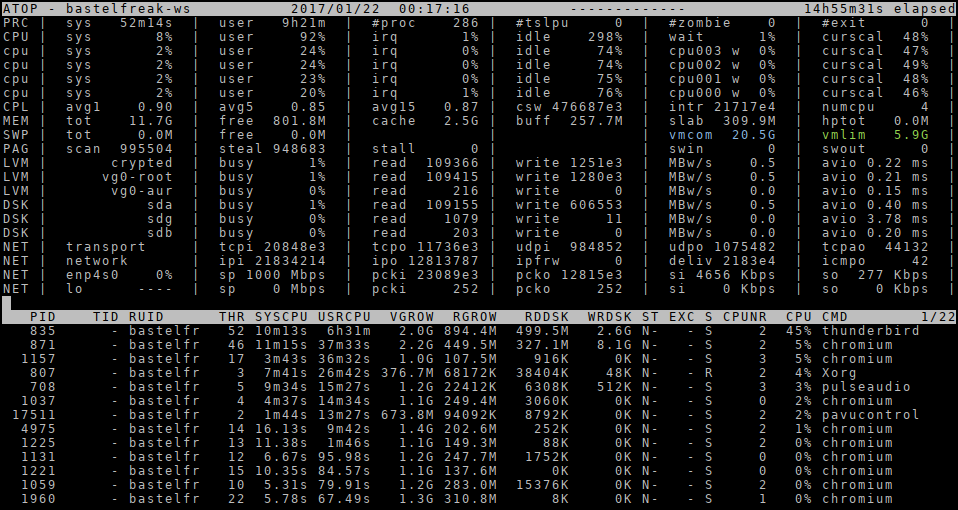
\includegraphics[width=1.0\textwidth]{../figures/atop_1.png}
  \caption{atop mit geringer Systemlast}
\label{figure:atop1}
\end{figure}

\begin{figure}
  \centering
  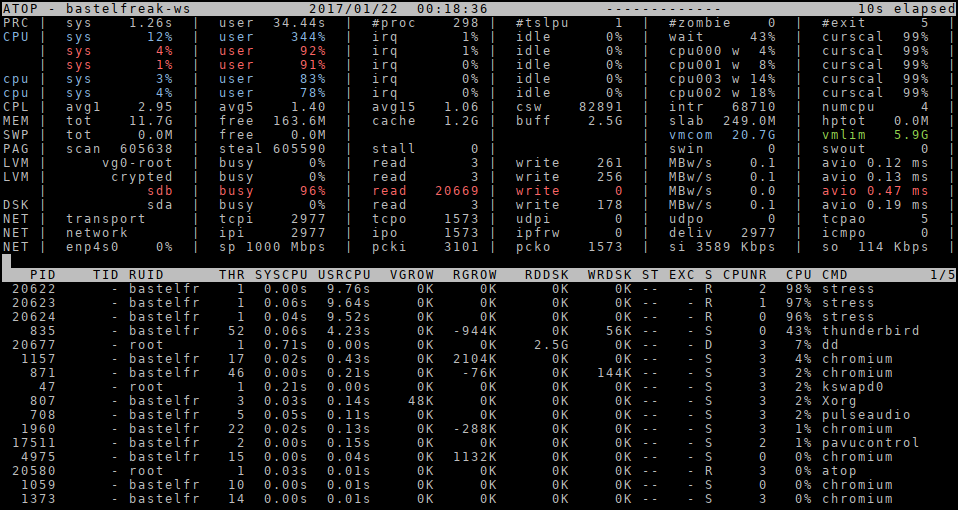
\includegraphics[width=1.0\textwidth]{../figures/atop_2.png}
  \caption{atop mit hoher CPU/Netzwerk Last}
\label{figure:atop2}
\end{figure}

\begin{figure}
  \centering
  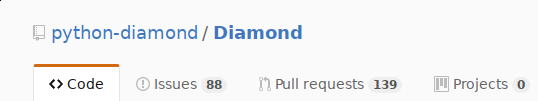
\includegraphics[width=1.0\textwidth]{../figures/diamond.png}
  \caption{Offene PRs und Issues im Diamond Projekt - 22.01.2017}
\label{figure:diamond}
\end{figure}
\FloatBarrier{}


\begin{listing}
  \inputminted[fontsize=\small]{text}{../listings/atop.txt}
  \caption{atop ASCII Logausgabe}
  \label{lst:atop}
\end{listing}
\begin{listing}
  \inputminted[breaklines]{js}{../listings/logstash-conf.txt}
  \caption{Logstash Konfigurationsdatei}
  \label{lst:logstash}
\end{listing}
\begin{listing}
  \inputminted{json}{../listings/facter.txt}
  \caption{Ausgabe von facter}
  \label{lst:facter}
\end{listing}
\begin{listing}
  \inputminted{puppet}{../listings/grafana-puppet.txt}
  \caption{Puppet Profil für Grafana Beispiel}
  \label{lst:grafana}
\end{listing}
\begin{listing}
  \inputminted{sql}{../listings/postgres-part-sample.txt}
  \caption{Manuelle Partitionierung Postgres}
  \label{lst:postgressample}
\end{listing}
\begin{listing}
  \inputminted{text}{../listings/output-unittest.txt}
  \caption{Test-Ausgabe der Unit-Tests}
  \label{lst:output-unittests}
\end{listing}
\begin{listing}
  \inputminted[breaklines]{ruby}{../listings/full-acceptance-test.txt}
  \caption{Vollständiger Akzeptanztest für das Modul collectd}
  \label{lst:collectd-test}
\end{listing}
\begin{listing}
  \inputminted{yaml}{../listings/def-centos.txt}
  \caption{Beispieldatei für eine Betriebssystem definition}
  \label{lst:def-centos}
\end{listing}


\newpage

\section{Erklärung}
Hiermit erklären wir, dass wir die Arbeit selbstständig verfasst und keine
anderen als die angegebenen Quellen und Hilfsmittel benutzt haben. Diese Arbeit
wurde keinem anderen Prüfungsausschuss in gleicher oder vergleichbarer Form
vorgelegt.

\vfill
{\centering
\renewcommand{\arraystretch}{0.9}
\begin{tabular}{p{0.25\textwidth}p{0.05\textwidth}p{0.25\textwidth}p{0.05\textwidth}p{0.25\textwidth}}
  \dotfill                    & & \dotfill                      & & \dotfill \\
  \centering\footnotesize{Tim Meusel}& & \centering\footnotesize{Marcel Reuter}& & \centering\footnotesize{Nikolai Luis}%
\end{tabular}
}

%%% Local Variables:
%%% mode: latex
%%% TeX-master: "thesis-de"
%%% End:
